\chapter{Constrained Least Squares}

\section{Karush-Kuhn-Tucker Conditions}

\begin{problem}
    \begin{equation}
\begin{array}{l}
\min _{x}\left\{f(x)=2 x_{1}^{2}+x_{2}^{2}\right\} \\
\text { s.t. } \quad h(x)=x_{1}+x_{2}-1=0
\end{array}
\end{equation}

直接利用无约束优化问题求解: 
\begin{equation} \nabla f(x)=\left[\begin{array}{l}4 x_{1} \\ 2 x_{2}\end{array}\right]=0 \Rightarrow x=\left[\begin{array}{l}0 \\ 0\end{array}\right] \end{equation}

显然不满足约束条件 $ x_{1}+x_{2}-1=0+0-1 \neq 0 $, 不是优化问题的解。
\end{problem}

由约束条件可得 $ x_{1}=1-x_{2} $ , 代入目标函数则有

\begin{equation} f(x)=3 x_{2}^{2}-4 x_{2}+2 \end{equation}
即当 $ \hat{x}_{2}=\frac{2}{3} $ 时,目标函数值最小,并有 $ \hat{x}_{1}=1-\hat{x}_{2}=\frac{1}{3} $ .

\begin{FigureCenter}{The Geometry of the problem}
    \label{fig:geometry-of-the-problem}
    

\tikzset{every picture/.style={line width=0.75pt}} %set default line width to 0.75pt        

\begin{tikzpicture}[x=0.75pt,y=0.75pt,yscale=-1,xscale=1]
%uncomment if require: \path (0,333); %set diagram left start at 0, and has height of 333

%Straight Lines [id:da5016924761517159] 
\draw    (240.45,208.11) -- (460.06,208.46) ;
\draw [shift={(463.06,208.46)}, rotate = 180.09] [fill={rgb, 255:red, 0; green, 0; blue, 0 }  ][line width=0.08]  [draw opacity=0] (8.93,-4.29) -- (0,0) -- (8.93,4.29) -- cycle    ;
%Straight Lines [id:da4228098452592868] 
\draw    (240.45,208.11) -- (240.26,50.64) ;
\draw [shift={(240.26,47.64)}, rotate = 449.93] [fill={rgb, 255:red, 0; green, 0; blue, 0 }  ][line width=0.08]  [draw opacity=0] (8.93,-4.29) -- (0,0) -- (8.93,4.29) -- cycle    ;
%Shape: Rectangle [id:dp4169105767030461] 
\draw  [dash pattern={on 0.84pt off 2.51pt}] (240.45,126.72) -- (279.2,126.72) -- (279.2,208.11) -- (240.45,208.11) -- cycle ;
%Straight Lines [id:da38972494470736385] 
\draw [color={rgb, 255:red, 74; green, 144; blue, 226 }  ,draw opacity=1 ][line width=2.25]    (240.91,88.18) -- (357.45,208.11) ;
%Straight Lines [id:da6148568898829554] 
\draw [color={rgb, 255:red, 152; green, 195; blue, 245 }  ,draw opacity=1 ][line width=2.25]    (271.9,120.08) -- (388.44,240) ;
%Straight Lines [id:da5253071245967558] 
\draw [color={rgb, 255:red, 152; green, 195; blue, 245 }  ,draw opacity=1 ][line width=2.25]    (205.39,51.63) -- (321.93,171.55) ;
%Straight Lines [id:da011458677930073602] 
\draw [color={rgb, 255:red, 184; green, 84; blue, 80 }  ,draw opacity=1 ][fill={rgb, 255:red, 184; green, 84; blue, 80 }  ,fill opacity=1 ][line width=1.5]    (240.91,88.18) -- (260.95,67.55) ;
\draw [shift={(263.74,64.68)}, rotate = 494.18] [fill={rgb, 255:red, 184; green, 84; blue, 80 }  ,fill opacity=1 ][line width=0.08]  [draw opacity=0] (11.61,-5.58) -- (0,0) -- (11.61,5.58) -- cycle    ;
%Straight Lines [id:da8455771801891709] 
\draw [color={rgb, 255:red, 245; green, 166; blue, 35 }  ,draw opacity=1 ][fill={rgb, 255:red, 184; green, 84; blue, 80 }  ,fill opacity=1 ][line width=1.5]    (279.2,126.72) -- (299.24,106.1) ;
\draw [shift={(302.03,103.23)}, rotate = 494.18] [fill={rgb, 255:red, 245; green, 166; blue, 35 }  ,fill opacity=1 ][line width=0.08]  [draw opacity=0] (11.61,-5.58) -- (0,0) -- (11.61,5.58) -- cycle    ;
%Shape: Ellipse [id:dp8656582545427394] 
\draw  [color={rgb, 255:red, 245; green, 166; blue, 35 }  ,draw opacity=1 ][dash pattern={on 5.63pt off 4.5pt}][line width=1.5]  (163.6,204.04) .. controls (163.6,150.27) and (195.41,106.68) .. (234.64,106.68) .. controls (273.87,106.68) and (305.68,150.27) .. (305.68,204.04) .. controls (305.68,257.81) and (273.87,301.4) .. (234.64,301.4) .. controls (195.41,301.4) and (163.6,257.81) .. (163.6,204.04) -- cycle ;

% Text Node
\draw (225.88,81.79) node [anchor=north west][inner sep=0.75pt]  [xscale=0.75,yscale=0.75]  {$1$};
% Text Node
\draw (159.43,103.67) node [anchor=north west][inner sep=0.75pt]  [xscale=0.75,yscale=0.75]  {$\hat{x}_{1} =\frac{2}{3}$};
% Text Node
\draw (254.9,212.59) node [anchor=north west][inner sep=0.75pt]  [xscale=0.75,yscale=0.75]  {$\hat{x}_{2} =\frac{1}{3}$};
% Text Node
\draw (451.96,210.8) node [anchor=north west][inner sep=0.75pt]  [xscale=0.75,yscale=0.75]  {$x_{1}$};
% Text Node
\draw (230.45,29.38) node [anchor=north west][inner sep=0.75pt]  [xscale=0.75,yscale=0.75]  {$x_{2}$};
% Text Node
\draw (347.29,210.72) node [anchor=north west][inner sep=0.75pt]  [xscale=0.75,yscale=0.75]  {$1$};
% Text Node
\draw (33.88,198.25) node [anchor=north west][inner sep=0.75pt]  [color={rgb, 255:red, 185; green, 126; blue, 27 }  ,opacity=1 ,xscale=0.75,yscale=0.75]  {$f( x) =2x_{1}^{2} +x_{2}^{2}$};
% Text Node
\draw (329.11,238.71) node [anchor=north west][inner sep=0.75pt]  [color={rgb, 255:red, 74; green, 144; blue, 226 }  ,opacity=1 ,xscale=0.75,yscale=0.75]  {$h( x) =x_{1} +x_{2} -1=0$};
% Text Node
\draw (305,84.4) node [anchor=north west][inner sep=0.75pt]  [xscale=0.75,yscale=0.75]  {$\textcolor[rgb]{0.96,0.65,0.14}{\nabla f(\hat{x})} =\lambda \textcolor[rgb]{0.72,0.33,0.31}{\nabla h(\hat{x} )}$};
% Text Node
\draw (255,45.4) node [anchor=north west][inner sep=0.75pt]  [color={rgb, 255:red, 184; green, 84; blue, 80 }  ,opacity=1 ,xscale=0.75,yscale=0.75]  {$\nabla h(\hat{x} )$};


\end{tikzpicture}
\end{FigureCenter}

注意到

$$ \nabla f(\hat{x})=\left[\begin{array}{l}4 \hat{x}_{1} \\ 2 \hat{x}_{2}\end{array}\right]=\left[\begin{array}{l}\frac{4}{3} \\ \frac{4}{3}\end{array}\right] $$

$$ \nabla h(\hat{x})=\left[\begin{array}{l}1 \\ 1\end{array}\right] $$

为了惩罚这个解未能满足约束条件, 引入\term{拉格朗日函数 (Lagrange Function)}
\begin{equation}
L(x, \lambda)=f(x)-\lambda h(x)=2 x_{1}^{2}+x_{2}^{2}+\lambda\left(1-x_{1}-x_{2}\right)
\end{equation}

对拉格朗日函数进行求导

\begin{equation} \left.\begin{array}{l}\frac{\partial L}{\partial x_{1}}=4 x_{1}-\lambda=0 \\ \frac{\partial L}{\partial x_{2}}=2 x_{2}-\lambda=0 \\ \frac{\partial L}{\partial \lambda}=1-x_{1}-x_{2}=0\end{array}\right \} \Rightarrow \hat{x}_{1}=\frac{1}{3}, \hat{x}_{2}=\frac{2}{3}, \hat{\lambda}=\frac{4}{3} \end{equation}

\begin{definition}[拉格朗日乘子法和Lagrange Functions]
    \begin{equation}\begin{aligned}
        \min _{x} / \max_{x}& f(x) \\
\text{ s.t. } & h_{i}(x)=0, i \in I \triangleq\{1, \cdots, p\} \\
&g_{j}(x) \leq 0, j \in J \triangleq\{1, \cdots, q\}
    \end{aligned}\end{equation}

$ \lambda_{i} \in \mathbb{R}, i \in {I}, u_{j} \in \mathbb{R}^{+}, j \in J $称为\term{拉格朗日乘子(Lagrange Multipliers)} .

引入拉格朗日函数 \begin{equation} L(x, \lambda, u)=f(x)-\sum_{i \in I} \lambda_{i} h_{i}(x)-\sum_{j \in J} u_{j} g_{j}(x)   \end{equation}

设$\lambda=\left[\begin{array}{c}\lambda_{1} \\ \vdots \\ \lambda_{p}\end{array}\right], u=\left[\begin{array}{c}u_{1} \\ \vdots \\ u_{q}\end{array}\right]$,$h(x),g(x)$假设可以视为一个向量。

则拉格朗日乘子式可写成


\begin{equation} L(x, \lambda, u)=f(x) - \lambda^T h(x) - u^T g(x)\end{equation}

拉格朗日乘子法求得的解要使拉格朗日函数的梯度为0.

\end{definition}

\begin{theorem}[拉格朗日函数求导]
    对拉格朗日函数进行求导,有

\begin{equation} \nabla_{x} L(x, \lambda, u)=\nabla_{x} f(x)-\sum_{i \in I} \lambda_{i} \nabla_{x} h_{i}(x)-\sum_{j \in J} u_{j} \nabla_{x} g_{j}(x)=0 \end{equation}

\begin{equation}\nabla_{x} f(x)=\sum_{i \in I} \lambda_{i} \nabla_{x} h_{i}(x)+\sum_{j \in J} u_{j} \nabla_{x} g_{j}(x)\end{equation}

    与图\ref{fig:geometry-of-the-problem}中的结论相符。
\end{theorem}

\begin{theorem}[Karush-Kuhn-Tucker Conditions] 
    对于优化问题

    \begin{equation}\begin{aligned}
        \min _{x} / \max_x &f(x) \\
\text{ s.t. } & h_{i}(x)=0, i \in I \triangleq\{1, \cdots, p\} \\
&g_{j}(x) \leq 0, j \in J \triangleq\{1, \cdots, q\}
    \end{aligned}\end{equation}
    
    KKT条件包括:
\begin{itemize}
    \item $\nabla_{x} L(x, \lambda, u)=\nabla_{x} f(x)-\sum_{i \in I} \lambda_{i} \nabla_{x} h_{i}(x)-\sum_{j \in J} u_{j} \nabla_{x} g_{j}(x)=0$
    \item $ h_{i}(x)=0, i \in I $
    \item $ \lambda_{i} h_{i}(x)=0, i \in I $
    \item $ g_{j}(x) \leq 0, j \in J $
    \item $ u_{j} g_{j}(x)=0, j \in J $
    \item $ u_{j} \geq 0, j \in J $
\end{itemize}
\end{theorem}


\subsection{An Example for Karush-Kuhn-Tucker Conditions}
   
\begin{problem}
    求解
\begin{equation}
\begin{aligned}
    \max _{x}&\left\{f(x)=20 x_{1}+10 x_{2}\right\} \\
  \text{ s.t. }  &   g_{1}(x)=x_{1}^{2}+x_{2}^{2} \leq 1 \\
  & g_{2}(x)=x_{1}+2 x_{2} \leq 2 \\
  &  g_{3}(x)=-x_{1} \leq 0 \\
    & g_{4}(x)=-x_{2} \leq 0 
\end{aligned}
\end{equation}
\end{problem}

\begin{FigureCenter}{An Example for Karush-Kuhn-Tucker Conditions}
    

\tikzset{every picture/.style={line width=0.75pt}} %set default line width to 0.75pt        

\begin{tikzpicture}[x=0.75pt,y=0.75pt,yscale=-1,xscale=1]
%uncomment if require: \path (0,300); %set diagram left start at 0, and has height of 300

%Straight Lines [id:da1344500183097299] 
\draw    (176.45,210.13) -- (450,210.92) ;
\draw [shift={(453,210.93)}, rotate = 180.17] [fill={rgb, 255:red, 0; green, 0; blue, 0 }  ][line width=0.08]  [draw opacity=0] (8.93,-4.29) -- (0,0) -- (8.93,4.29) -- cycle    ;
%Straight Lines [id:da9389602487873245] 
\draw    (176.45,210.13) -- (176.26,52.66) ;
\draw [shift={(176.26,49.66)}, rotate = 89.93] [fill={rgb, 255:red, 0; green, 0; blue, 0 }  ][line width=0.08]  [draw opacity=0] (8.93,-4.29) -- (0,0) -- (8.93,4.29) -- cycle    ;
%Straight Lines [id:da10284635814725096] 
\draw [color={rgb, 255:red, 74; green, 144; blue, 226 }  ,draw opacity=1 ][line width=0.75]  [dash pattern={on 0.84pt off 2.51pt}]  (176.91,90.2) -- (410.44,210.13) ;
%Straight Lines [id:da17435619545267356] 
\draw [color={rgb, 255:red, 152; green, 195; blue, 245 }  ,draw opacity=1 ][line width=2.25]    (176.91,90.2) -- (259,132.09) ;
%Straight Lines [id:da18154884528370974] 
\draw [color={rgb, 255:red, 184; green, 84; blue, 80 }  ,draw opacity=1 ][fill={rgb, 255:red, 184; green, 84; blue, 80 }  ,fill opacity=1 ][line width=1.5]    (209.91,95.2) -- (276.22,72.39) ;
\draw [shift={(280,71.09)}, rotate = 161.02] [fill={rgb, 255:red, 184; green, 84; blue, 80 }  ,fill opacity=1 ][line width=0.08]  [draw opacity=0] (11.61,-5.58) -- (0,0) -- (11.61,5.58) -- cycle    ;
%Shape: Free Drawing [id:dp709786381310392] 
\draw  [color={rgb, 255:red, 245; green, 166; blue, 35 }  ,draw opacity=1 ][line width=2.25] [line join = round][line cap = round] (259,131.93) .. controls (263.45,131.93) and (265.36,142.29) .. (268,144.93) .. controls (283.47,160.4) and (289,182.44) .. (289,209.93) ;


% Text Node
\draw (161.88,83.81) node [anchor=north west][inner sep=0.75pt]  [xscale=0.75,yscale=0.75]  {$1$};
% Text Node
\draw (293.96,176.83) node [anchor=north west][inner sep=0.75pt]  [xscale=0.75,yscale=0.75]  {$\textcolor[rgb]{0.96,0.65,0.14}{g}\textcolor[rgb]{0.96,0.65,0.14}{_{1}}\textcolor[rgb]{0.96,0.65,0.14}{(}\textcolor[rgb]{0.96,0.65,0.14}{x}\textcolor[rgb]{0.96,0.65,0.14}{)}\textcolor[rgb]{0.96,0.65,0.14}{=x}\textcolor[rgb]{0.96,0.65,0.14}{_{1}^{2}}\textcolor[rgb]{0.96,0.65,0.14}{+x}\textcolor[rgb]{0.96,0.65,0.14}{_{2}^{2}}\textcolor[rgb]{0.96,0.65,0.14}{-1=0}$};
% Text Node
\draw (166.45,31.4) node [anchor=north west][inner sep=0.75pt]  [xscale=0.75,yscale=0.75]  {$x_{2}$};
% Text Node
\draw (283.29,213.74) node [anchor=north west][inner sep=0.75pt]  [xscale=0.75,yscale=0.75]  {$1$};
% Text Node
\draw (216,54.42) node [anchor=north west][inner sep=0.75pt]  [color={rgb, 255:red, 184; green, 84; blue, 80 }  ,opacity=1 ,xscale=0.75,yscale=0.75]  {$\textcolor[rgb]{0.72,0.33,0.31}{\nabla f}\textcolor[rgb]{0.72,0.33,0.31}{(}\textcolor[rgb]{0.72,0.33,0.31}{\hat{x}}\textcolor[rgb]{0.72,0.33,0.31}{)}$};
% Text Node
\draw (278,120.82) node [anchor=north west][inner sep=0.75pt]  [xscale=0.75,yscale=0.75]  {$\left(\frac{4}{5} ,\frac{3}{5}\right)$};
% Text Node
\draw (404.29,213.74) node [anchor=north west][inner sep=0.75pt]  [xscale=0.75,yscale=0.75]  {$2$};
% Text Node
\draw (197,162.42) node [anchor=north west][inner sep=0.75pt]  [xscale=0.75,yscale=0.75] [align=left] {可行域};
% Text Node
\draw (235.96,94.83) node [anchor=north west][inner sep=0.75pt]  [xscale=0.75,yscale=0.75]  {$\textcolor[rgb]{0.29,0.56,0.89}{g}\textcolor[rgb]{0.29,0.56,0.89}{_{2}}\textcolor[rgb]{0.29,0.56,0.89}{(}\textcolor[rgb]{0.29,0.56,0.89}{x}\textcolor[rgb]{0.29,0.56,0.89}{)}\textcolor[rgb]{0.29,0.56,0.89}{=x}\textcolor[rgb]{0.29,0.56,0.89}{_{1}}\textcolor[rgb]{0.29,0.56,0.89}{+2x}\textcolor[rgb]{0.29,0.56,0.89}{_{2}}\textcolor[rgb]{0.29,0.56,0.89}{-2=0}$};


\end{tikzpicture}
\end{FigureCenter}


对拉格朗日函数求导
\begin{equation} \nabla_{x} L(x, u)=\nabla_{x} f(x)-u_{1} \nabla_{x} g_{1}(x)-u_{2} \nabla_{x} g_{2}(x)-u_{3} \nabla_{x} g_{3}(x)-u_{4} \nabla_{x} g_{4}(x)=0, u_{j} \geq 0 \end{equation}

计算各个部分,可得
\begin{equation} \nabla_{x} f(x)=\left[\begin{array}{c}20 \\ 10\end{array}\right], \nabla_{x} g_{1}(x)=\left[\begin{array}{c}2 x_{1} \\ 2 x_{2}\end{array}\right], \nabla_{x} g_{2}(x)=\left[\begin{array}{l}1 \\ 2\end{array}\right], \nabla_{x} g_{3}(x)=\left[\begin{array}{l}-1 \\ 0\end{array}\right], \nabla_{x} g_{4}(x)=\left[\begin{array}{l}0 \\ -1\end{array}\right]\end{equation}

检测边界条件,注意约束条件$u_{j} \geq 0$,可知
\begin{equation} \nabla_{x} f(x)=u_{1} \nabla_{x} g_{1}(x), \nabla_{x} f(x) \neq u_{2} \nabla_{x} g_{2}(x), \nabla_{x} f(x) \neq u_{3} \nabla_{x} g_{3}(x), \nabla_{x} f(x) \neq u_{4} \nabla_{x} g_{4}(x) \end{equation}

即$\nabla_{x} f(x)$只可能是$u_{1} \nabla_{x} g_{1}(x)$的线性组合。

所以
\begin{equation} u_{2}=u_{3}=u_{4}=0, \quad u_{1} \neq 0 \end{equation}

即

\begin{equation}
\begin{aligned}
    \nabla_{x} f(x)&=u_{1} \nabla_{x} g_{1}(x)\\
\left[\begin{array}{c}
20 \\
10
\end{array}\right]&=u_{1}\left[\begin{array}{c}
2 x_{1} \\
2 x_{2}
\end{array}\right]\\
x_{1}&=2 x_{2} 
\end{aligned}
\end{equation}

由KKT条件得$ u_{j} g_{j}(x)=0, j \in J $.由于$ u_{2}=u_{3}=u_{4}=0, \quad u_{1} \neq 0 $,所以$g_1(x) = 0$.


将上式代入

\begin{equation}g_{1}(x)=x_{1}^{2}+x_{2}^{2}-1=5 x_{2}^{2}-1=0\end{equation}


由于 $ x_{2} \geq 0 $, 可得 $x = \left[\begin{array}{l}x_{1} \\ x_{2}\end{array}\right]=\frac{\sqrt{5}}{5}\left[\begin{array}{l}2 \\ 1\end{array}\right], u_{1}=5 \sqrt{5} $.

\section{优化问题:最小范数优化问题}

\begin{problem}

\begin{equation}\begin{aligned}
    \min _{x} &\|x\|_{2}^{2}\\
   \text{s.t.} &C x=d 
\end{aligned}\end{equation}

矩阵 $C \in \mathbb{R}^{p \times n} $, 向量 $ d \in \mathbb{R}^{p} $.
\end{problem}


在大多数应用中 $ p<n,  C x=d $ 是一个\textbf{欠定方程}.这时,$C x=d$表示为一条直线。它的几何意义是在直线 $ C x=d $ 中,寻找范数最小的解。

假如$p = n$,$C x=d$表示一个点。

\begin{FigureCenter}{最小范数优化问题($p < n$)}
    

\tikzset{every picture/.style={line width=0.75pt}} %set default line width to 0.75pt        

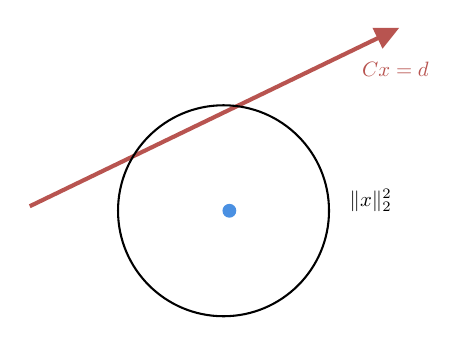
\begin{tikzpicture}[x=0.75pt,y=0.75pt,yscale=-1,xscale=1]
%uncomment if require: \path (0,300); %set diagram left start at 0, and has height of 300

%Straight Lines [id:da6117902046112789] 
\draw [color={rgb, 255:red, 184; green, 84; blue, 80 }  ,draw opacity=1 ][fill={rgb, 255:red, 184; green, 84; blue, 80 }  ,fill opacity=1 ][line width=1.5]    (199,160.65) -- (373.4,76.41) ;
\draw [shift={(377,74.67)}, rotate = 154.22] [fill={rgb, 255:red, 184; green, 84; blue, 80 }  ,fill opacity=1 ][line width=0.08]  [draw opacity=0] (11.61,-5.58) -- (0,0) -- (11.61,5.58) -- cycle    ;
%Shape: Circle [id:dp3140562285855766] 
\draw   (241.53,162.82) .. controls (241.53,134.75) and (264.28,112) .. (292.35,112) .. controls (320.42,112) and (343.18,134.75) .. (343.18,162.82) .. controls (343.18,190.89) and (320.42,213.65) .. (292.35,213.65) .. controls (264.28,213.65) and (241.53,190.89) .. (241.53,162.82) -- cycle ;
%Shape: Circle [id:dp5255822841062723] 
\draw  [color={rgb, 255:red, 74; green, 144; blue, 226 }  ,draw opacity=1 ][fill={rgb, 255:red, 74; green, 144; blue, 226 }  ,fill opacity=1 ] (292.35,162.82) .. controls (292.35,161.26) and (293.62,160) .. (295.18,160) .. controls (296.74,160) and (298,161.26) .. (298,162.82) .. controls (298,164.38) and (296.74,165.65) .. (295.18,165.65) .. controls (293.62,165.65) and (292.35,164.38) .. (292.35,162.82) -- cycle ;

% Text Node
\draw (358,90) node [anchor=north west][inner sep=0.75pt]  [color={rgb, 255:red, 184; green, 84; blue, 80 }  ,opacity=1 ,xscale=0.75,yscale=0.75]  {$Cx=d$};
% Text Node
\draw (352,151.4) node [anchor=north west][inner sep=0.75pt]  [xscale=0.75,yscale=0.75]  {$\| x\| _{2}^{2}$};


\end{tikzpicture}
\end{FigureCenter}



假设矩阵$C$行向量线性无关时,有:
\begin{itemize}
    \item 对任意一个 $ {d}, C x=d $ 至少有一个解;
    \item 矩阵$C$为宽的或者方的 $ (p \leq n) $;
    \item 当 $ p<n $,有无穷多个解。
\end{itemize}

\subsection{最小范数优化问题的例子}

\begin{problem}
    矩阵 $ C \in \mathbb{R}^{2 \times 10} $, 向量 $ d \in \mathbb{R}^{2} $ :

\begin{equation}Cx=d\end{equation}

\begin{equation}\displaystyle \underbrace{\left[\begin{array}{ c c c c c }
    19/2 & 17/2 & 15/2 & \cdots  & 1/2\\
    1 & 1 & 1 & \cdots  & 1
    \end{array}\right]}_{C} x=\underbrace{\left[\begin{array}{ l }
    1\\
    0
    \end{array}\right]}_{d}\end{equation}
\end{problem}

这个方程只有一组含有两个非0元素的解。

\begin{equation}
x=\left[\begin{array}{c}
1 \\
-1 \\
0 \\
\vdots \\
0
\end{array}\right], \quad x=\left[\begin{array}{c}
0 \\
1 \\
-1 \\
\vdots \\
0
\end{array}\right], \cdots
\end{equation}

\section{优化问题:点到线的最短距离}

\begin{problem}
    给定点 $ a \neq 0 $ ,点到线最短距离问题:
\begin{equation}
\begin{array}{ll}
\min _{x} & \|x-a\|_{2}^{2} \\
\text { s.t. } & C x=d
\end{array}
\end{equation}

\end{problem}

\begin{FigureCenter}{点到线的最短距离}
    

\tikzset{every picture/.style={line width=0.75pt}} %set default line width to 0.75pt        

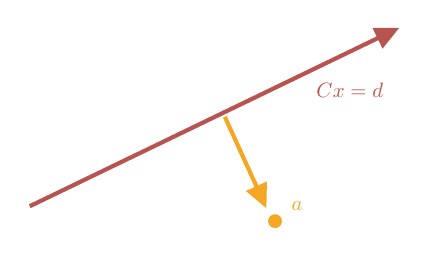
\begin{tikzpicture}[x=0.75pt,y=0.75pt,yscale=-1,xscale=1]
%uncomment if require: \path (0,300); %set diagram left start at 0, and has height of 300

%Straight Lines [id:da9999289567232588] 
\draw [color={rgb, 255:red, 184; green, 84; blue, 80 }  ,draw opacity=1 ][fill={rgb, 255:red, 184; green, 84; blue, 80 }  ,fill opacity=1 ][line width=1.5]    (241,170.65) -- (415.4,86.41) ;
\draw [shift={(419,84.67)}, rotate = 154.22] [fill={rgb, 255:red, 184; green, 84; blue, 80 }  ,fill opacity=1 ][line width=0.08]  [draw opacity=0] (11.61,-5.58) -- (0,0) -- (11.61,5.58) -- cycle    ;
%Shape: Circle [id:dp5553159381717454] 
\draw  [color={rgb, 255:red, 245; green, 166; blue, 35 }  ,draw opacity=1 ][fill={rgb, 255:red, 245; green, 166; blue, 35 }  ,fill opacity=1 ] (356.35,177.82) .. controls (356.35,176.26) and (357.62,175) .. (359.18,175) .. controls (360.74,175) and (362,176.26) .. (362,177.82) .. controls (362,179.38) and (360.74,180.65) .. (359.18,180.65) .. controls (357.62,180.65) and (356.35,179.38) .. (356.35,177.82) -- cycle ;
%Straight Lines [id:da5135858807849654] 
\draw [color={rgb, 255:red, 245; green, 166; blue, 35 }  ,draw opacity=1 ][fill={rgb, 255:red, 184; green, 84; blue, 80 }  ,fill opacity=1 ][line width=1.5]    (335,127.57) -- (353.34,167.93) ;
\draw [shift={(355,171.57)}, rotate = 245.56] [fill={rgb, 255:red, 245; green, 166; blue, 35 }  ,fill opacity=1 ][line width=0.08]  [draw opacity=0] (11.61,-5.58) -- (0,0) -- (11.61,5.58) -- cycle    ;

% Text Node
\draw (378,110) node [anchor=north west][inner sep=0.75pt]  [color={rgb, 255:red, 184; green, 84; blue, 80 }  ,opacity=1 ,xscale=0.75,yscale=0.75]  {$Cx=d$};
% Text Node
\draw (366,167.4) node [anchor=north west][inner sep=0.75pt]  [xscale=0.75,yscale=0.75]  {$\textcolor[rgb]{0.96,0.65,0.14}{a}$};


\end{tikzpicture}
\end{FigureCenter}


令 $ y=x-a $, 则点到线的最短距离问题, 可等价为最小范数问题:

\begin{problem}
    \begin{equation}
\begin{array}{ll}
\min _{y} & \|y\|_{2}^{2} \\
\text { s. t. } & C y=d-C a
\end{array}
\end{equation}
\end{problem}

则 $ x=y+a $ 是点到线最短距离问题的解。

\section{最小范数优化问题求解推导}

\begin{problem}
    \begin{equation}
\begin{array}{ll}
\min _{x}& \frac{1}{2}\|x\|_{2}^{2} \\
\text { s.t. }& C x=d
\end{array}
\end{equation}

求其最优解。
\end{problem}

引入拉格朗日函数
\begin{equation}
L(x, \lambda)=\frac{1}{2}\|x\|_{2}^{2}-\lambda^{T}(C x-d)
\end{equation}

\begin{remark}
    $\lambda$是一个向量。
\end{remark}

对拉格朗日函数求导
\begin{equation}
\nabla_{x} L(x, \lambda)=x-C^{T} \lambda=0 \Rightarrow x=C^{T} \lambda
\end{equation}

由矩阵$C$行线性无关可得
\begin{equation}
C x=C C^{T} \lambda=d \Rightarrow \lambda=\left(C C^{T}\right)^{-1} d
\end{equation}

则有
\begin{equation}
\hat{x}=C^{T} \lambda=C^{T}\left(C C^{T}\right)^{-1} d=C^{\dagger} d
\end{equation}

以上得到的是$\hat{x}=C^{\dagger} d$是问题最优解的必要条件。还需要证明它是最优解。

\begin{theorem}
    $\hat{x}=C^{\dagger} d$是问题最优解。
\end{theorem}

\begin{proof}
    1.首先证明解 $ \hat{x} $ 满足等式 $ \hat{x}=C^{T} \lambda=C^{T}\left(C C^{T}\right)^{-1} d=C^{\dagger} d $.

\begin{equation}
C \hat{x}=C C^{T}\left(C C^{T}\right)^{-1} d=d
\end{equation}

2. 在 $ C x=d, x \neq \hat{x} $ 的情况下

\begin{equation}
\begin{aligned}
\hat{x}^{T}(x-\hat{x}) &=d^{T}\left(C C^{T}\right)^{-1} C(x-\hat{x}) \\
&=d^{T}\left(C C^{T}\right)^{-1}(C x-C \hat{x}) \\
&=d^{T}\left(C C^{T}\right)^{-1}(d-d) \\
&=0
\end{aligned}
\end{equation}

3.在 $ C x=d, x \neq \hat{x} $ 的情况下,证明 $ \|x\|_{2}^{2}>\|\hat{x}\|_{2}^{2} $.

\begin{equation}
\begin{aligned}
\|x\|_{2}^{2} &=\|\hat{x}+x-\hat{x}\|_{2}^{2} \\
&=\|\hat{x}\|_{2}^{2}+2 \hat{x}^{T}(x-\hat{x})+\|x-\hat{x}\|_{2}^{2} \\
&=\|\hat{x}\|_{2}^{2}+\|x-\hat{x}\|_{2}^{2} \\
&>\|\hat{x}\|_{2}^{2}
\end{aligned}
\end{equation}
\end{proof}

\section{QR分解求解最小范数优化问题}

对矩阵 $ C^{T} \in \mathbb{R}^{n \times p} $ 进行 $ Q R $ 分解, $ C^{T}=Q R $
\begin{equation}
\begin{aligned}
\hat{x} &=C^{T}\left(C C^{T}\right)^{-1} d \\
&=Q R\left(R^{T} Q^{T} Q R\right)^{-1} d \\
&=Q R\left(R^{T} R\right)^{-1} d \\
&=Q \left(R^{-1}\right)^T d
\end{aligned}
\end{equation}

\begin{algorithm}[htbp]
    \caption{QR分解求解最小范数优化问题}
    \KwIn{QR分解得到的矩阵$Q$、$R$,向量$d$}
    \KwOut{$\hat{x}$}
    求解$R^T z=d$ \;
    求解$\hat{x} = Qz$\;
    
\end{algorithm}

\begin{proof}
    \begin{equation}\displaystyle \begin{aligned}
    \hat{x} & =Q\underbrace{\left( R^{T}\right)^{-1} d}_{\textcolor[rgb]{0.72,0.33,0.31}{z}}\\
    \textcolor[rgb]{0.72,0.33,0.31}{z} & =\left( R^{T}\right)^{-1} d\Rightarrow R^{T}\textcolor[rgb]{0.72,0.33,0.31}{z} =d\\
    \hat{x} & =Q\textcolor[rgb]{0.72,0.33,0.31}{z}
    \end{aligned}\end{equation}
\end{proof}


\subsection{QR分解求解最小范数优化问题的复杂度}

总复杂度:$ \approx 2 n p^{2} $ flops

\begin{itemize}
    \item 矩阵 $ C^{T}=Q R $ 分解, $ C^{T}=Q R\left(2 n p^{2}  \text{ flops}\right) $
    \item 回代法求解 $ R^{T} z=d\left(p^{2} \text{ flops} \right) $
    \item 计算 $ \hat{x}=Q z(2 n p \text{ flops} ) $
\end{itemize}



\subsection{QR分解求解最小范数优化问题的例子}

\begin{example}
    \begin{equation}
C=\left[\begin{array}{cccc}
1 & -1 & 1 & 1 \\
1 & 0 & 1 / 2 & 1 / 2
\end{array}\right], \quad d=\left[\begin{array}{l}
0 \\
1
\end{array}\right]
\end{equation}
对矩阵 $ C^{T} $ 进行 $ Q R $ 分解, $ C^{T}=Q R $
\begin{equation}
\left[\begin{array}{cc}
1 & 1 \\
-1 & 0 \\
1 & 1 / 2 \\
1 & 1 / 2
\end{array}\right]=\left[\begin{array}{cc}
1 / 2 & 1 / \sqrt{2} \\
-1 / 2 & 1 / \sqrt{2} \\
1 / 2 & 0 \\
1 / 2 & 0
\end{array}\right]\left[\begin{array}{cc}
2 & 1 \\
0 & 1 / \sqrt{2}
\end{array}\right]
\end{equation}
通过回代法求解 $ R^{T} z=d $
\begin{equation}
\left[\begin{array}{cc}
2 & 0 \\
1 & 1 / \sqrt{2}
\end{array}\right]\left[\begin{array}{l}
z_{1} \\
z_{2}
\end{array}\right]=\left[\begin{array}{l}
0 \\
1
\end{array}\right]
\end{equation}

解得$
 z_{1}=0, z_{2}=\sqrt{2}
$.

可得 $ \hat{x}=Q z=(1,1,0,0) $
\end{example}

\section{最小二乘法约束问题}

\begin{problem}[分段多项式拟合问题]
    \begin{equation}\begin{aligned}
        \min _{x} &\|A x-b\|_{2}^{2} \\
        \text{s.t.} & Cx =d 
    \end{aligned}\end{equation}

    矩阵 $ {A} \in \mathbb{R}^{m \times n}, {C} \in \mathbb{R}^{p \times n} $, 向量 $ {b} \in \mathbb{R}^{m}, d \in \mathbb{R}^{p} $
\end{problem}


% todo (2021-11-25 13:02): figure

在大多数应用中 $ p<n, C x=d $ 是一个欠定方程。它的几何意义是在直线 $ C x=d $ 中,寻找 $ \|A x-b\|_{2}^{2} $ 最小的解。(此时$\|A x-b\|_{2}^{2}$表示一个椭圆).

特殊情况:

\begin{itemize}
    \item 当 $ {p}=0 $ 时,则其转化为无约束的最小二乘法问题。
    \item 当 $ {A}=I, b=0 $ 时,则其为最小范数问题。
\end{itemize}




\section{优化问题:分段多项式拟合问题}

\begin{problem}
    假设样本点 $ \left(x_{1}, y_{1}\right), \ldots,\left(x_{N}, y_{N}\right) \in \mathbb{R}^{2} $ ,有 \begin{equation} x_{1}, \ldots, x_{M} \leq a , x_{M+1}, \ldots, x_{N}>a\end{equation}

    设$ {d} $ 阶多项式 

    \begin{equation}
    \begin{aligned}
        f(x)&=\theta_{1}+\theta_{2} x+\cdots+\theta_{d} x^{d-1}\\
        g(x)&=\theta_{d+1}+\theta_{d+2} x \ldots+\theta_{2 d} x^{d-1}
    \end{aligned}
    \end{equation}

    两个多项式 $ f(x), g(x) $ 对于样本点 $ \left(x_{1}, y_{1}\right), \ldots,\left(x_{N}, y_{N}\right) $ 进行拟合

    \begin{equation}
    \begin{array}{l}
    f\left(x_{i}\right) \approx y_{i}, x_{i} \leq a \\
    g\left(x_{i}\right) \approx y_{i}, x_{i}>a
    \end{array}
    \end{equation}

    拟合要求:函数值和导数值必须在分段位置 $ a $ 连续
    \begin{equation}
    f(a)=g(a), f^{\prime}(a)=g^{\prime}(a)
    \end{equation}
\end{problem}

对于$
\left\{
    \begin{array}{l}
f\left(x_{i}\right) \approx y_{i}, x_{i} \leq a \\
g\left(x_{i}\right) \approx y_{i}, x_{i}>a
\end{array}
\right.
$,可以构造矩阵

\begin{notation}
    \begin{equation}\displaystyle A=\left[\begin{array}{ c c c c c c c c }
        \textcolor[rgb]{0.72,0.33,0.31}{\boldsymbol{1}} & \textcolor[rgb]{0.72,0.33,0.31}{\boldsymbol{x_{1}}} & \textcolor[rgb]{0.72,0.33,0.31}{\boldsymbol{\cdots }} & \textcolor[rgb]{0.72,0.33,0.31}{\boldsymbol{x_{1}^{d-1}}} & 0 & 0 & \cdots  & 0\\
        \vdots  & \vdots  &  & \vdots  & \vdots  & \vdots  &  & \vdots \\
        1 & x_{M} & \cdots  & x_{M}^{d-1} & 0 & 0 & \cdots  & 0\\
        0 & 0 & \cdots  & 0 & 1 & x_{M+1} & \cdots  & x_{M+1}^{d-1}\\
        \vdots  & \vdots  &  & \vdots  & \vdots  & \vdots  &  & \vdots \\
        0 & 0 & \cdots  & 0 & 1 & x_{N} & \cdots  & x_{N}^{d-1}
        \end{array}\right] ,\theta =\left[\begin{array}{ c }
        \textcolor[rgb]{0.72,0.33,0.31}{\boldsymbol{\theta _{1}}}\\
        \textcolor[rgb]{0.72,0.33,0.31}{\boldsymbol{\vdots }}\\
        \textcolor[rgb]{0.72,0.33,0.31}{\boldsymbol{\theta _{d}}}\\
        \theta _{d+1}\\
        \vdots \\
        \theta _{2d}
        \end{array}\right] ,b=\left[\begin{array}{ c }
        \textcolor[rgb]{0.72,0.33,0.31}{\boldsymbol{y_{1}}}\\
        \vdots \\
        y_{M}\\
        y_{M+1}\\
        \vdots \\
        y_{N}
        \end{array}\right]\end{equation}
\end{notation}

则可以转化为

\begin{equation} A \theta \approx b \end{equation}

对于约束条件$f(a)=g(a), f^{\prime}(a)=g^{\prime}(a)$,可以构造矩阵

\begin{notation}
    \begin{equation} C=\left[\begin{array}{cccccccc}1 & a & \cdots & a^{d-1} & -1 & -a & \cdots & -a^{d-1} \\ 0 & 1 & \cdots & (d-1) a^{d-2} & 0 & -1 & \cdots & -(d-1) a^{d-2}\end{array}\right], 
    \theta =\left[\begin{array}{ c }
        \theta _{1}\\
        \vdots \\
        \theta _{d}\\
        \theta _{d+1}\\
        \vdots \\
        \theta _{2d}
        \end{array}\right], 
    d=\left[\begin{array}{l}0 \\ 0\end{array}\right] \end{equation}
\end{notation}


所以

\begin{equation} C \theta=d \end{equation}

对于分段多项式拟合问题

\begin{problem}[分段多项式拟合问题]
    假设样本点 $ \left(x_{1}, y_{1}\right), \ldots,\left(x_{N}, y_{N}\right) \in \mathbb{R}^{2} $ ,有 $ x_{1}, \ldots, x_{M} \leq a $, $ x_{M+1}, \ldots, x_{N}>a $.

     \begin{equation}\begin{array}{ll}\min _{\theta} & \sum_{i=1}^{M}\left(f\left(x_{i}\right)-y_{i}\right)^{2}+\sum_{i=M+1}^{N}\left(g\left(x_{i}\right)-y_{i}\right)^{2} \\ \text { s.t. } & f(a)=g(a), f^{\prime}(a)=g^{\prime}(a)\end{array}\end{equation}
\end{problem}

最终可以转换成矩阵形式

\begin{problem}[分段多项式拟合问题(矩阵形式)]
    \begin{equation}\begin{aligned}
        \min _{\theta}&\|A \theta-b\|_{2}^{2}\\
       \text{s.t.} & C \theta=d
    \end{aligned}\end{equation}

\end{problem}

\section{先验假设}

\begin{proposition}
    \label{prop:assumption-1}

    堆叠矩阵的列向量线性无关
\begin{equation}
\left[\begin{array}{l}
A \\
C
\end{array}\right] \in \mathbb{R}^{(m+p) \times n}
\end{equation}
\end{proposition}

\begin{proposition}
    \label{prop:assumption-2}
    矩阵 $ C \in \mathbb{R}^{p \times n} $行线性无关

\end{proposition}

假设 1 是一个比 $ A $ 可右逆更弱的条件。 

假设$ p \leq n \leq m+p $.

\section{优化问题:最小二乘法的带约束KKT条件}

\begin{problem}
    \begin{equation}\begin{aligned}
        \min _{x} & \frac{1}{2}\|A x-b\|_{2}^{2}\\
        s.t. & C x=d
    \end{aligned}\end{equation}
\end{problem}


引入拉格朗日函数
\begin{equation}
L(x, z)=\frac{1}{2}\|A x-b\|_{2}^{2}-z^{T}(d-C x), z \in \mathbb{R}^{p}
\end{equation}

对拉格朗日函数求导


\begin{equation}
    \label{eqn:kkt-deriavative}
    \begin{array}{l}
\nabla_{x} L(x, z)=A^{T}(A x-b)+C^{T} z=0 \\
\nabla_{z} L(x, z)=C x-d=0
\end{array}
\end{equation}



\begin{remark}
    使用矩阵导数

    \begin{equation} \begin{aligned} \frac{\partial}{\partial {X}} \operatorname{Tr}\left({X}^{T} {B X}\right) &={B X}+{B}^{T} {X} \\ \frac{\partial}{\partial {X}} \operatorname{Tr}\left({B X X}^{T}\right) &={B X}+{B}^{T} {X} \\ \frac{\partial}{\partial {X}} \operatorname{Tr}\left({X X}^{T} {B}\right) &={B X}+{B}^{T} {X} \\ \frac{\partial}{\partial {X}} \operatorname{Tr}\left({X B X}^{T}\right) &={X B}^{T}+{X B} \\ \frac{\partial}{\partial {X}} \operatorname{Tr}\left({B X}^{T} {X}\right) &={X B}^{T}+{X B} \\ \frac{\partial}{\partial {X}} \operatorname{Tr}\left({X}^{T} {X B}\right) &={X B}^{T}+{X B} \end{aligned} \end{equation}

    可以求得

    \begin{equation}\begin{aligned}
        \frac{\partial \frac{1}{2} \| Ax-b\| _{2}^{2}}{\partial x} & =\frac{\partial \frac{1}{2}\left( x^{T} A^{T} Ax-2x^{T} A^{T} b+b^{T} b\right)}{\partial x}\\
         & =\frac{\partial \frac{1}{2}\operatorname{tr}\left( x^{T} A^{T} Ax\right)}{\partial x} -\frac{\partial x^{T} A^{T} b}{\partial x}\\
         & =\frac{1}{2} \cdotp 2A^{T} Ax-A^{T} b\\
         & =A^{T}( Ax-b)
        \end{aligned}\end{equation}
\end{remark}

可以转换成矩阵形式

\begin{equation} \left[\begin{array}{cc}A^{T} A & C^{T} \\ {C} & 0\end{array}\right]\left[\begin{array}{l}x \\ z\end{array}\right]=\left[\begin{array}{l}A^{T} b \\ d\end{array}\right] \end{equation}

\section{KKT最优条件}

\begin{problem}
    \begin{equation}\begin{aligned}
        \min _{x} & \frac{1}{2}\|A x-b\|_{2}^{2}\\
        s.t. & C x=d
    \end{aligned}\end{equation}
\end{problem}

\begin{theorem}[优化条件的Karush-Kuhn-Tucker(KKT)等式]
    令 $ \hat{x} $ 是上述约束优化问题的解,则有
\begin{equation}
\left[\begin{array}{cc}
A^{T} A & C^{T} \\
C& 0
\end{array}\right]\left[\begin{array}{l}
\hat{x} \\
z
\end{array}\right]=\left[\begin{array}{l}
A^{T} b \\
d
\end{array}\right],\left[\begin{array}{l}
\hat{x} \\
z
\end{array}\right] \in \mathbb{R}^{n+p}
\end{equation}

则它是最优解。
\end{theorem}


特殊情况:

\begin{itemize}
    \item 最小二乘法问题:当 $ p=0 $ 时,即为正规方程 $ A^{T} A \hat{x}=A^{T} b $
    \item 最小范数问题: 当 $ A=I, b=0 $ 时,可以推导得到 $ C \hat{x}=b, \hat{x}+C^{T} z=0 $
\end{itemize}


\begin{proof}
    假设 $ x $ 满足 $ C x=d,(\hat{x}, z) $ 满足KKT等式$ \left[\begin{array}{cc}A^{T} A & C^{T} \\ {C} & 0\end{array}\right]\left[\begin{array}{l}x \\ z\end{array}\right]=\left[\begin{array}{l}A^{T} b \\ d\end{array}\right] $的定义,即$x$是另一个解。

    所以有

    \begin{equation}\begin{aligned}
        \| Ax-b\| _{2}^{2} & =\| A(x-\hat{x} )+A\hat{x} -b\| _{2}^{2}\\
         & =\| A(x-\hat{x} )\| _{2}^{2} +\| A\hat{x} -b\| _{2}^{2} +2(x-\hat{x} )^{T} A^{T} (A\hat{x} -b)\\
         & =\| A(x-\hat{x} )\| _{2}^{2} +\| A\hat{x} -b\| _{2}^{2} -\underbrace{2(x-\hat{x} )^{T}}_{\textcolor[rgb]{0.96,0.65,0.14}{(Cx=C\hat{x} =d)}}\underbrace{C^{T} z}_{\textcolor[rgb]{0.72,0.33,0.31}{ \left( A^{T} A\hat{x} +C^{T} z=A^{T} b\right)}}\\
         & =\| A(x-\hat{x} )\| _{2}^{2} +\| A\hat{x} -b\| _{2}^{2}\\
         & \geq \| A\hat{x} -b\| _{2}^{2}
        \end{aligned}\end{equation}

    \begin{remark}
        $x$ 和 $\hat{x}$ 都是KKT等式的解,所以 $Cx = C \hat{x} = d$.

        由拉格朗日函数求导\ref{eqn:kkt-deriavative},有
        \begin{equation}\ A^{T} A\hat{x} +C^{T} z=A^{T} b\end{equation}
        
    \end{remark}

        所以$\hat{x}$是最优解。
\end{proof}

\begin{theorem}[KKT等式最优解的唯一性]
    最优解$ \hat{x} $ 是唯一的。
\end{theorem}

\begin{proof}
    假设矩阵$A$列线性无关, $C$行线性无关,即
    \begin{equation}
    \begin{aligned}
    A^{T} A(\hat{x}-x) &=0 \Rightarrow x=\hat{x} \quad (A^TA 可逆) \\
    C^{T}(\hat{z}-z) &=0 \Rightarrow \hat{z}=z \\
    \end{aligned}
    \end{equation}

    所以对于方程
    \begin{equation}A^{T} A \hat{x}+C^{T} z =A^{T} b\end{equation}

    $\left[\begin{array}{l}x \\ z\end{array}\right]$也是唯一的。
\end{proof}
        
\begin{theorem}
    如果矩阵$A$列线性无关, $C$行线性无关,则矩阵
\begin{equation}
\left[\begin{array}{cc}
A^{T} A & C^{T} \\
{C} & 0
\end{array}\right]
\end{equation}
为非奇异矩阵。  
\end{theorem}

\begin{proof}
    \begin{equation} \begin{aligned}\left[\begin{array}{cc}A^{T} A & C^{T} \\ {C} & 0\end{array}\right]\left[\begin{array}{c}x \\ z\end{array}\right]=0 & \Rightarrow x^{T}\left(A^{T} A x+C^{T} z\right)=0, C x=0 \\ & \Rightarrow\|A x\|_{2}^{2}+(C x)^{T} z=\|A x\|_{2}^{2}=0, C x=0 \\ & \Rightarrow A x=0, C x=0 \\ & \Rightarrow x=0 \quad (A\text {列线性无关}) \end{aligned} \end{equation}

    由于 $ A^{T} A x+C^{T} {z}=0 $, 则当 $ x=0 $ 时,有 $ {z}=0 $ . 
    
    所以$C$行线性无关。
\end{proof}

\begin{theorem}
    如果矩阵$A$列线性无关和 $ C $ 行线性无关不同时成立,则矩阵
\begin{equation}
\left[\begin{array}{cc}
A^{T} A & C^{T} \\
{C} & 0
\end{array}\right]
\end{equation}
为奇异矩阵。
\end{theorem}

\begin{proof}
    如果 $ {A} $ 列线性相关,则存在 $ x \neq 0 $, 使得 $ A x=0 $, 则

    \begin{equation}
    \left[\begin{array}{cc}
    A^{T} A & C^{T} \\
    {C} & 0
    \end{array}\right]\left[\begin{array}{l}
    x \\
    0
    \end{array}\right]=0
    \end{equation}

    如果 $ C $ 行线性相关,则存在 $ z \neq 0 $, 使得 $ C^{T} z=0 $, 则

    \begin{equation}
    \left[\begin{array}{cc}
    A^{T} A & C^{T} \\
    {C} & 0
    \end{array}\right]\left[\begin{array}{l}
    0 \\
    {z}
    \end{array}\right]=0
    \end{equation}

    因此该矩阵为奇异矩阵。
\end{proof}


\section{LU分解求解KKT最优条件}

\begin{problem}
    \begin{equation}\begin{aligned}
        \min _{x} & \frac{1}{2}\|A x-b\|_{2}^{2}\\
        s.t. & C x=d
    \end{aligned}\end{equation}

    \begin{equation}
\left[\begin{array}{cc}
A^{T} A & C^{T} \\
C & 0
\end{array}\right]\left[\begin{array}{l}
x \\
z
\end{array}\right]=\left[\begin{array}{c}
A^{T} b \\
d
\end{array}\right]
\end{equation}

求其最优解。
\end{problem}



\begin{algorithm}[htbp]
    \caption{LU分解求解KKT最优条件}
    \KwIn{矩阵$\left[\begin{array}{cc}
        A^{T} A & C^{T} \\
        C & 0
        \end{array}\right]$、向量$\left[\begin{array}{l}
            x \\
            z
            \end{array}\right]$}
    \KwOut{向量$\left[\begin{array}{l}
        x \\
        z
        \end{array}\right]$}
    计算 $ H=A^{T} A $\;
    计算 $ c=A^{T} b $ \;
    LU分解求解\begin{equation}
    \left[\begin{array}{cc}
    H & C^{T} \\
    C & 0
    \end{array}\right]\left[\begin{array}{l}
    x \\
    z
    \end{array}\right]=\left[\begin{array}{l}
    c \\
    d
    \end{array}\right]
    \end{equation}\;
\end{algorithm}

\subsection{LU分解求解KKT最优条件的时间复杂度}

\begin{theorem}
    用LU分解法求解下列线性方程 
\begin{equation}
\left[\begin{array}{cc}
H & C^{T} \\
C & 0
\end{array}\right]\left[\begin{array}{l}
x \\
z
\end{array}\right]=\left[\begin{array}{l}
c \\
d
\end{array}\right]
\end{equation}

需要的时间复杂度是$ \frac{2}{3}(p+n)^{3} $ flops.
\end{theorem}

第一步的时间复杂度是$2 m n^{2}  \text{flops} $,第二步的时间复杂度是$2 {mn} $ flops,总时间复杂度为$ 2 m n^{2}+\frac{2}{3}(p+n)^{3} $ flops .

\section{QR分解求解KKT最优条件}

\begin{problem}
    \begin{equation}\begin{aligned}
        \min _{x} & \frac{1}{2}\|A x-b\|_{2}^{2}\\
        s.t. & C x=d
    \end{aligned}\end{equation}

    它的矩阵形式是
    \begin{equation}
\left[\begin{array}{cc}
A^{T} A & C^{T} \\
C & 0
\end{array}\right]\left[\begin{array}{l}
x \\
z
\end{array}\right]=\left[\begin{array}{c}
A^{T} b \\
d
\end{array}\right]
\end{equation}

求其最优解。
\end{problem}


由于 $ \hat{x} $ 满足 $ C \hat{x}=d $ ,则有 \begin{equation}\displaystyle \textcolor[rgb]{0.72,0.33,0.31}{C^{T} C\hat{x}} =\textcolor[rgb]{0.96,0.65,0.14}{C^{T} d}\end{equation} 

列出拉格朗日函数
\begin{equation}
L(x, z)=\frac{1}{2}\|A x-b\|_{2}^{2}-z^{T}(d-C x)
\end{equation}

由KKT条件可得
\begin{equation}\begin{aligned}
    \nabla _{x} L(x,z) & =A^{T} (A\hat{x} -b)+\textcolor[rgb]{0.96,0.65,0.14}{C^{T} z} +\textcolor[rgb]{0.72,0.33,0.31}{C^{T} C\hat{x}} -\textcolor[rgb]{0.96,0.65,0.14}{C^{T} d} =0\\
     & \Rightarrow \left( A^{T} A+\textcolor[rgb]{0.72,0.33,0.31}{C^{T} C}\right)\hat{x} +\textcolor[rgb]{0.96,0.65,0.14}{C^{T} (z-d)} =A^{T} b\\
    \nabla _{z} L(x,z) & =C\hat{x} -d=0
    \end{aligned}
\end{equation}

令 $ w=z-d $ , KKT条件写成矩阵形式
\begin{equation}
\left[\begin{array}{cc}
A^{T} A+C^{T} C & C^{T} \\
C & 0
\end{array}\right]\left[\begin{array}{l}
\hat{x} \\
w
\end{array}\right]=\left[\begin{array}{c}
A^{T} b \\
d
\end{array}\right]
\end{equation}

假设 1($ \left[\begin{array}{l}A \\ C\end{array}\right] $ 列向量无关),命题\ref{prop:assumption-1}保证了 $ A^{T} A+C^{T} C $ 是非奇异的,即存在以下 $ Q R $ 因子分解

\begin{equation} \left[\begin{array}{l}A \\ C\end{array}\right]=Q R=\left[\begin{array}{l}Q_{1} \\ Q_{2}\end{array}\right] R=\left[\begin{array}{l}Q_{1} R \\ Q_{2} R\end{array}\right] \end{equation}

代入QR分解,可得
\begin{equation}
\left[\begin{array}{cc}
R^{T} R & R^{T} Q_{2}^{T} \\
Q_{2} R & 0
\end{array}\right]\left[\begin{array}{c}
\hat{x} \\
w
\end{array}\right]=\left[\begin{array}{c}
R^{T} Q_{1}^{T} b \\
d
\end{array}\right]
\end{equation}

将第一个方程两边乘 $ R^{-T} $ 和并令变量 $ y=R \hat{x} $ ,可得
\begin{equation}\displaystyle \left[\begin{array}{ c c }
    \left(\textcolor[rgb]{0.72,0.33,0.31}{\left( R^{T}\right)^{-1}} R^{T}\right) R & \left(\textcolor[rgb]{0.72,0.33,0.31}{\left( R^{T}\right)^{-1}} R^{T}\right) Q_{2}^{T}\\
    Q_{2} R & 0
    \end{array}\right]\left[\begin{array}{ c }
    \hat{x}\\
    w
    \end{array}\right] =\left[\begin{array}{ c }
    \left(\textcolor[rgb]{0.72,0.33,0.31}{\left( R^{T}\right)^{-1}} R^{T}\right) Q_{1}^{T} b\\
    d
    \end{array}\right]\end{equation}

\begin{equation}\displaystyle \left[\begin{array}{ c c }
    \textcolor[rgb]{0.25,0.46,0.02}{R} & Q_{2}^{T}\\
    Q_{2}\textcolor[rgb]{0.25,0.46,0.02}{R} & 0
    \end{array}\right]\left[\begin{array}{ c }
    \textcolor[rgb]{0.25,0.46,0.02}{\hat{x}}\\
    w
    \end{array}\right] =\left[\begin{array}{ c }
    Q_{1}^{T} b\\
    d
    \end{array}\right]\end{equation}

\begin{equation}\displaystyle \left[\begin{array}{ c c }
    I & Q_{2}^{T}\\
    Q_{2} & 0
    \end{array}\right]\left[\begin{array}{ c }
    \textcolor[rgb]{0.25,0.46,0.02}{R\hat{x}}\\
    w
    \end{array}\right] =\left[\begin{array}{ c }
    Q_{1}^{T} b\\
    d
    \end{array}\right]\end{equation}

\begin{equation}\displaystyle \left[\begin{array}{ c c }
    I & Q_{2}^{T}\\
    Q_{2} & 0
    \end{array}\right]\left[\begin{array}{ c }
    \textcolor[rgb]{0.25,0.46,0.02}{y}\\
    w
    \end{array}\right] =\left[\begin{array}{ c }
    Q_{1}^{T} b\\
    d
    \end{array}\right]\end{equation}


矩阵 $ C=Q_{2} R \Rightarrow Q_{2}=C R^{-1}, Q_{2} $ 行线性无关
\begin{equation}
Q_{2}^{T} u=R^{-T} C^{T} u=0  \Rightarrow  C^{T} u=0 \Rightarrow  u=0
\end{equation}
因为 $ C $ 行线性无关的(假设2 (\ref{prop:assumption-2}))。

利用 $ Q_{2}^{T} $ 的 $ Q R $ 分解来求解
\begin{equation}
\left[\begin{array}{cc}
I & Q_{2}^{T} \\
Q_{2} & 0
\end{array}\right]\left[\begin{array}{l}
y \\
w
\end{array}\right]=\left[\begin{array}{c}
Q_{1}^{T} b \\
d
\end{array}\right]
\end{equation}

方程第1行可得 $ y=Q_{1}^{T} b-Q_{2}^{T} w $ ,并代入第二行
\begin{equation}
Q_{2} y=d \Rightarrow Q_{2} Q_{2}^{T} w=Q_{2} Q_{1}^{T} b-d
\end{equation}

用QR分解 $ Q_{2}^{T}=\tilde{Q} \tilde{R} $ 来解这个关于 $ w $ 的方程:
\begin{equation}
\tilde{R}^{T} \tilde{R} w=\tilde{R}^{T} \tilde{Q}^{T} Q_{1}^{T} b-d
\end{equation}

上式可以简化为:
\begin{equation}
\tilde{R} w=\tilde{Q}^{T} Q_{1}^{T} b-\tilde{R}^{-T} d
\end{equation}

\begin{equation} \left[\begin{array}{cc}A^{T} A+C^{T} C & C^{T} \\ C & 0\end{array}\right]\left[\begin{array}{c}\hat{x} \\ w\end{array}\right]=\left[\begin{array}{c}A^{T} b \\ d\end{array}\right] \quad \tilde{R} w=\tilde{Q}^{T} Q_{1}^{T} b-\tilde{R}^{-T} d \end{equation}

算法过程见\ref{algo:qr-kkt}.

\begin{algorithm}[htbp]
    \caption{QR分解求解KKT最优条件}
    \KwIn{$\begin{aligned}
        \min _{x} & \frac{1}{2}\|A x-b\|_{2}^{2}\\
        s.t. & C x=d
    \end{aligned}$中的$A$, $C$, $d$}
    \KwOut{最优解$\hat{x}$}
    \label{algo:qr-kkt}
    计算两个QR分解
\begin{equation}
\left[\begin{array}{l}
A\\
C
\end{array}\right]=\left[\begin{array}{l}
Q_{1} \\
Q_{2}
\end{array}\right] R, Q_{2}^{T}=\tilde{Q} \tilde{R}
\end{equation}\;
用前代法求解 $ \tilde{R}^{T} u=d $ \;
计算 $ c=\tilde{Q}^{T} Q_{1}^{T} b-u $\;
用回代法求解 $ \tilde{R} w=c $ \;
计算 $ y=Q_{1}^{T} b-Q_{2}^{T} w $\;
用回代法计算 $ R \hat{x}=y_{\circ} $\;

\end{algorithm}

总时间复杂度: QR分解有 $ 2(p+m) n^{2}+2 n p^{2} $ 次flops.


\section{KKT最优条件求解复杂度:QR vs LU}

假设 $ p<n $ :

\begin{itemize}
    \item LU复杂度: $ 2 m n^{2}+(2 / 3)(p+n)^{3}<2 m n^{2}+(16 / 3) n^{3} $
    \item QR复杂度: $ 2(p+m) n^{2}+2 n p^{2}<2 m n^{2}+4 n^{3} $
\end{itemize}

稳定性: QR分解避免直接计算 $ A^{T} {A}$.

\section[Supplement Material: Karush-Kuhn-Tucker (KKT)条件]{Supplement Material: Karush-Kuhn-Tucker (KKT)条件\footnote{Cited from \url{https://zhuanlan.zhihu.com/p/38163970}.}}

\subsection{等式约束优化问题}

\begin{problem}[等式约束优化问题]
    给定一个目标函数 $ f: \mathbb{R}^{n} \rightarrow \mathbb{R} $, 我们希望找到 $ {x} \in \mathbb{R}^{n} $, 在满足约束条件 $ g({x})=0 $ 的前提下, 使得 $ f({x}) $ 有最小值

    \begin{equation}
\begin{array}{ll}
\min & f({x}) \\
\text { s.t. } & g({x})=0
\end{array}
\end{equation}
\end{problem}

为方便分析, 假设 $ f $ 与 $ g $ 是连续可导函数。 Lagrange乘数法是等式约束优化问题的典型解法。定义

\begin{definition}[Lagrangian函数]
    \begin{equation}
L({x}, \lambda)=f({x})+\lambda g({x})
\end{equation}
\end{definition}

其中 $ \lambda $ 称为\term{Lagrange乘数}. 

\begin{theorem}
    Lagrange乘数法将原本的约束优化问题转换成等价的无约束优化问题
\begin{equation}
\min _{{x}, \lambda} L({x}, \lambda)
\end{equation}
\end{theorem}

\begin{theorem}[拉格朗日乘子法最优解必要条件]
    计算 $ L $ 对 $ {x} $ 与 $ \lambda $ 的偏导数并设为零,可得最优解的必要条件:
\begin{equation}
\begin{array}{l}
\nabla_{{x}} L=\dfrac{\partial L}{\partial {x}}=\nabla f+\lambda \nabla g={0} \\
\\
\nabla_{\lambda} L=\dfrac{\partial L}{\partial \lambda}=g({x})=0
\end{array}
\end{equation}

其中第一式为\term{定常方程式(stationary equation)}, 第二式为\term{约束条件}.
\end{theorem}


解开上面 $ n+1 $ 个方程式可 得 $ L({x}, \lambda) $ 的驻点(stationary point) $ {x}^{\star} $ 以及 $ \lambda $ 的值(正负数皆可能).

\subsection{不等式约束优化问题}

接下来我们将约束等式 $ g({x})=0 $ 推广为不等式 $ g({x}) \leq 0 $ .考虑这个问题

\begin{problem}[不等式约束优化问题]

\begin{equation}
\begin{array}{ll}
\min & f({x}) \\
\text { s.t. } & g({x}) \leq 0
\end{array}
\end{equation}

约束不等式 $ g({x}) \leq 0 $ 称为\term{原始可行性(primal feasibility)}, 据此我们定义\term{可行域(feasible region)} $ K=\{ {x} \in \mathbb{R}^{n} \mid g({x}) \leq 0 \}$.
\end{problem}

假设 $ {x}^{\star} $ 为满足约束条件的最佳解, 分开两种情况讨论:

\begin{itemize}
    \item $ g\left({x}^{*}\right)<0 $, 最佳解位于 $ K $ 的内部, 称为内部解(interior solution), 这时约束条件是\term{无效的 (inactive)};
    \item $ g\left({x}^{*}\right)=0 $, 最佳解落在 $ K $ 的边界, 称为边界解(boundary solution), 此时约束条件是\term{有效的 (active)}.
\end{itemize}

这两种情况的最佳解具有不同的必要条件。

\begin{itemize}
    \item 内部解:在约束条件无效的情形下, $ g({x}) $ 不起作用, 约束优化问题退化为无约束优化问题, 因此驻点 $ {x}^{\star} $ 满足 $ \nabla f={0} $ 且 $ \lambda=0 $ .
    \item 边界解:在约束条件有效的情形下, 约束不等式变成等式 $g({x})=0$, 这与前述Lagrange乘数法的情况相同。
\end{itemize}

对于边界解,我们可以证明

\begin{theorem}
    驻点 ${x}^{\star}$ 发生于 $\nabla f \in \operatorname{span} \nabla g$.
\end{theorem}
换句话说, 

\begin{corollary}
    存在 $\lambda$ 使得 $\nabla f=-\lambda \nabla g$.

    注意这里 $\lambda$ 的正负号是有其意义的。
\end{corollary}

因为我们希望最小化 $f$, 梯度 $\nabla f$ (函数 $f$ 在 点 ${x}$ 的最陡上升方向)应该指向可行域 $K$ 的内部(因为最优解最小值是在边界取得的), 但 $\nabla g$ 指向 $K$ 的外部(即 $g({x})>0$ 的区域, 因为你的约束是小于等于0), 因此 $\lambda \geq 0$, 称为\term{对偶可行性(dual feasibility).}

因此, 不论是内部解或边界解, $\lambda g({x})=0$ 恒成立, 称为\term{互补松弛性(complementary slackness)}.

整合上述两种情况, 

\begin{theorem}[Karush-Kuhn-Tucker (KKT)条件]
    最佳解的必要条件包括:Lagrangian函数 $L({x}, \lambda)$ 的定常方程式、 原始可行性、对偶可行性,以及互补松弛性:
\begin{equation}
\begin{aligned}
\nabla_{{x}} L &=\nabla f+\lambda \nabla g={0} \\
g({x}) & \leq 0 \\
\lambda & \geq 0 \\
\lambda g({x}) &=0
\end{aligned}
\end{equation}
这些条件合称为\term{Karush-Kuhn-Tucker (KKT)条件}.

如果我们要最大化 $f({x})$ 且受限于 $g({x}) \leq 0$, 那么对偶可行性要改成 $\lambda \leq 0$ .
\end{theorem}


上面结果可推广至多个约束等式与约束不等式的情况。考虑标准约束优化问题(或称非线性规划):

\begin{definition}[标准约束优化问题(非线性规划)]
    \begin{equation}
\begin{array}{ll}
\min & f({x}) \\
\text { s.t. } & g_{j}({x})=0, \quad j=1, \ldots, m \\
& h_{k}({x}) \leq 0, \quad k=1, \ldots, p
\end{array}
\end{equation}
\end{definition}

\begin{theorem}[标准约束优化的KKT条件]
    定义Lagrangian 函数
\begin{equation}
L\left({x},\left\{\lambda_{j}\right\},\left\{\mu_{k}\right\}\right)=f({x})+\sum_{j=1}^{m} \lambda_{j} g_{j}({x})+\sum_{k=1}^{p} \mu_{k} h_{k}({x})
\end{equation}
其中 $ \lambda_{j} $ 是对应 $ g_{j}({x})=0 $ 的Lagrange乘数, $ \mu_{k} $ 是对应 $ h_{k}({x}) \leq 0 $ 的Lagrange乘数(或称KKT 乘数). 

KKT条件包括
\begin{equation}
\begin{aligned}
\nabla_{{x}} L &={0} \\
g_{j}({x}) &=0, \quad j=1, \ldots, m \\
h_{k}({x}) & \leq 0 \\
\mu_{k} & \geq 0 \\
\mu_{k} h_{k}({x}) &=0, \quad k=1, \ldots, p
\end{aligned}
\end{equation}

\end{theorem}

\subsection{拉格朗日乘子法的例子}

\begin{problem}

    考虑这个问题
\begin{equation}
\begin{array}{ll}
\min & x_{1}^{2}+x_{2}^{2} \\
\text { s.t. } & x_{1}+x_{2}=1 \\
& x_{2} \leq \alpha
\end{array}
\end{equation}
其中 $ \left(x_{1}, x_{2}\right) \in \mathbb{R}^{2}, \alpha $ 为实数。
\end{problem}

写出Lagrangigan函数
\begin{equation}
L\left(x_{1}, x_{2}, \lambda, \mu\right)=x_{1}^{2}+x_{2}^{2}+\lambda\left(1-x_{1}-x_{2}\right)+\mu\left(x_{2}-\alpha\right)
\end{equation}

KKT 方程组如下:
\begin{equation}
\begin{aligned}
\frac{\partial L}{\partial x_{i}} &=0, \quad i=1,2 \\
x_{1}+x_{2} &=1 \\
x_{2}-\alpha & \leq 0 \\
\mu & \geq 0 \\
\mu\left(x_{2}-\alpha\right) &=0
\end{aligned}
\end{equation}
求偏导可得 $ \frac{\partial L}{\partial x_{1}}=2 x_{1}-\lambda=0 $ 且 $ \frac{\partial L}{\partial x_{2}}=2 x_{2}-\lambda+\mu=0 $, 分别解出 $ x_{1}=\frac{\lambda}{2} $ 且 $ x_{2}=\frac{\lambda}{2}-\frac{\mu}{2} $ .代入约束等式 $ x_{1}+x_{2}=\lambda-\frac{\mu}{2}=1 $ 或 $ \lambda=\frac{\mu}{2}+1 $ .合并上面结果,
\begin{equation}
x_{1}=\frac{\mu}{4}+\frac{1}{2}, \quad x_{2}=-\frac{\mu}{4}+\frac{1}{2}
\end{equation}

最后再加入约束不等式 $ -\frac{\mu}{4}+\frac{1}{2} \leq \alpha $ 或 $ \mu \geq 2-4 \alpha $ .分开三种情况讨论。

\begin{enumerate}
    \item $ \alpha>\frac{1}{2} $ : 不难验证 $ \mu=0>2-4 \alpha $ 满足所有的KKT条件, 约束不等式是无效的, $ x_{1}^{\star}=x_{2}^{\star}=\frac{1}{2} $ 是内部解,目标函数的极小值是 $ \frac{1}{2}$.
    \item $ \alpha=\frac{1}{2} $ : 如同 $ 1, \quad \mu=0=2-4 \alpha $ 满足所有的KKT条件, $ \quad x_{1}^{\star}=x_{2}^{\star}=\frac{1}{2} $ 是边界解, 因为 $ x_{2}^{\star}=\alpha $.
    \item $ \alpha<\frac{1}{2} $ : 这时约束不等式是有效的, $ \mu=2-4 \alpha>0 $, 则 $ x_{1}^{\star}=1-\alpha $ 且 $ x_{2}^{\star}=\alpha $, 目标函数的极小值是 $ (1-\alpha)^{2}+\alpha^{2} $.
\end{enumerate}

\section[Supplement Material: 浅谈最优化问题的KKT条件]{Supplement Material: 浅谈最优化问题的KKT条件\footnote{Cited from \url{https://zhuanlan.zhihu.com/p/26514613}.}}


\begin{theorem}[KKT条件]
    对于具有等式和不等式约束的一般优化问题
\begin{equation}
\begin{aligned}
&\min f({x}) \\
\text { s.t. }& g_{j}({x}) \leq 0(j=1,2, \cdots, m) \\
&h_{k}({x})=0(k=1,2, \cdots, l)
\end{aligned}
\end{equation}
KKT 条件给出了判断 $ {x}^{*} $ 是否为最优解的\textbf{必要条件}, 即:
\begin{equation}
\left\{\begin{array}{l}
\frac{\partial f}{\partial x_{i}}+\sum_{j=1}^{m} \mu_{j} \frac{\partial g_{j}}{\partial x_{i}}+\sum_{k=1}^{l} \lambda_{k} \frac{\partial h_{k}}{\partial x_{i}}=0,(i=1,2, \ldots, n) \\
h_{k}({x})=0,(k=1,2, \cdots, l) \\
\mu_{j} g_{j}({x})=0,(j=1,2, \cdots, m) \\
\mu_{j} \geq 0
\end{array}\right.
\end{equation}
\end{theorem}


\subsection{等式约束优化问题}

等式约束优化问题是指

\begin{problem}[等式约束优化问题]
    \begin{equation}
\begin{array}{l}
\min f\left(x_{1}, x_{2}, \ldots, x_{n}\right) \\
\text { s.t. } h_{k}\left(x_{1}, x_{2}, \ldots, x_{n}\right)=0
\end{array}
\end{equation}
\end{problem}


我们令 $ L({x}, \lambda)=f({x})+\sum_{k=1}^{l} \lambda_{k} h_{k}({x}) $, 函数 $ L(x, y) $ 称为\term{Lagrange函数}, 参数 $ \lambda $ 称为\term{Lagrange乘子}.

再联立方程组: 
\begin{equation} \left\{\begin{array}{l}\frac{\partial L}{\partial x_{i}}=0(i=1,2, \cdots, n) \\ \frac{\partial L}{\partial \lambda_{k}}=0(k=1,2, \cdots, l)\end{array}\right. \end{equation}

得到的解为可能极值点,由于我们用的是必要条件,具体是否为极值点需根据问题本身的具体情况检验。 这个方程组称为\textbf{等式约束的极值必要条件}.

上式我们对 $ n $ 个 $ x_{i} $ 和 $ l $ 个 $ \lambda_{k} $ 分别求偏导, 回想一下在\term{无约束优化问题} 
\begin{equation} f\left(x_{1}, x_{2}, \ldots, x_{n}\right)=0 \end{equation} 
中, 我们根据极值的必要条件, 分别令 $ \frac{\partial f}{\partial x_{i}}=0 $, 求出可能的极值点。 

因此可以联想到:等式约束下的 Lagrange乘数法引入了 $ l $ 个Lagrange乘子,或许我们可以\textbf{把 $ \lambda_{k} $ 也看作优化变量}( $ x_{i} $ 就叫做\term{优化变量})。 相当于将优化变量个数增加到 $ (n+l) $ 个, $ x_{i} $ 与 $ \lambda_{k} $ 一视同仁, 均为优化变量, 均对它们求偏导。

\subsection{不等式约束优化问题}

以上我们讨论了等式约束的情形,接下来我们来介绍不等式约束的优化问题。

我们先给出其主要思想:\textbf{转化}的思想——\textbf{将不等式约束条件变成等式约束条件}.具体做法是\textbf{引入}\term{松弛变量}.松弛变量也是优化变量,也需要一视同仁求偏导。

具体而言, 我们先看一个一元函数的例子:

\begin{example}
    \begin{equation}\begin{aligned}
        \min& f(x)\\
    \text { s.t. }& g_{1}(x)=a-x \leq 0\\
    &g_{2}(x)=x-b \leq 0
    \end{aligned} \end{equation}
\end{example}

\begin{remark}
    优化问题中,我们必须求得一个确定的值,因此不妨令所有的不等式均取到等号,即 $ \leq $ 的情况。
\end{remark}


对于约束 $ g_{1} $ 和 $ g_{2} $, 我们分别引入两个松弛变量 $ a_{1}^{2} $ 和 $ b_{1}^{2} $, 得到 $ h_{1}\left(x, a_{1}\right)=g_{1}+a_{1}^{2}=0 $ 和 $ h_{2}\left(x, b_{1}\right)=g_{2}+b_{1}^{2}=0 $. 

\begin{remark}
    注意, 这里直接加上平方项 $ a_{1}^{2} 、 b_{1}^{2} $ 而非 $ a_{1} 、 b_{1} $, 是因为 $ g_{1} $ 和 $ g_{2} $ 这两个 不等式的左边必须加上一个正数才能使不等式变为等式。 若只加上 $ a_{1} $ 和 $ b_{1} $, 又会引入新的约束 $ a_{1} \geq 0 $ 和 $ b_{1} \geq 0 $, 这不符合我们的意愿。
\end{remark}


\begin{equation}\begin{aligned}
    g_1(x) &= a - x \le 0 \\
    g_2(x) &= x - b \le 0
\end{aligned} \Rightarrow \begin{aligned}
    &h_{1}\left(x, a_{1}\right)=g_{1}(x)+a_{1}^{2}=a-x+a_{1}^{2}=0\\
    &h_{2}\left(x, b_{1}\right)=g_{2}(x)+b_{1}^{2}=x-b+b_{1}^{2}=0
\end{aligned}\end{equation}


由此我们将不等式约束转化为了等式约束, 并得到Lagrange函数
\begin{equation}
L\left(x, a_{1}, b_{1}, \mu_{1}, \mu_{2}\right)=f(x)+\mu_{1}\left(a-x+a_{1}^{2}\right)+\mu_{2}\left(x-b+b_{1}^{2}\right)
\end{equation}
我们再按照等式约束优化问题(极值必要条件)对其求解, 联立方程
\begin{equation}
\left\{\begin{array}{l}
\dfrac{\partial F}{\partial x}=\dfrac{\partial f}{\partial x}+\mu_{1} \dfrac{d g_{1}}{d x}+\mu_{2} \dfrac{d g_{2}}{d x}=\dfrac{d f}{d x}-\mu_{1}+\mu_{2}=0 \\
\dfrac{\partial F}{\partial \mu_{1}}=g_{1}+a_{1}^{2}=0, \\ 
\dfrac{\partial F}{\partial \mu_{2}}=g_{2}+b_{1}^{2}=0 \\
\dfrac{\partial F}{\partial a_{1}}=2 \mu_{1} a_{1}=0, \\ 
\dfrac{\partial F}{\partial b_{1}}=2 \mu_{2} b_{1}=0 \\
\mu_{1} \geq 0, \quad \mu_{2} \geq 0
\end{array}\right.
\end{equation}

\begin{remark}
    对于不等式约束前的乘子, 我们要求其大于等于 0. ($\mu_{1} \geq 0, \mu_{2} \geq 0$)
\end{remark}

得出方程组后, 便开始动手解它。 看到第3行的两式 $\mu_{1} a_{1}=0$ 和 $\mu_{1} a_{1}=0$ 比较简单, 我们就从它们入手吧。

对于 $\mu_{1} a_{1}=0$, 我们有两种情况:

情形1 $: \quad \mu_{1}=0, a_{1} \neq 0$

此时由于乘子 $\mu_{1}=0$, 因此 $g_{1}$ 与其相乘为零, 可以理解为约束 $g_{1}$ 不起作用, 且有 $g_{1}(x)=a-x<0 .$

情形2: $\quad \mu_{1} \geq 0, a_{1}=0$

此时 $g_{1}(x)=a-x=0$ 且 $\mu_{1}>0$, 可以理解为约束 $g_{1}$ 起作用, 且有 $g_{1}(x)=0$.

合并情形 1 和情形 2 得: \textbf{$\mu_{1} g_{1}=0$, 且在约束起作用时 $\mu_{1}>0, g_{1}(x)=0$; 约束不起作用时 $\mu_{1}=0, g_{1}(x)<0 .$}

同样地, 分析 $\mu_{2} b_{1}=0$, 可得出约束 $g_{2}$ 起作用和不起作用的情形, 并分析得到 $\mu_{2} g_{2}=0$.

由此, 
\begin{theorem}[一元一次优化式的KKT条件]
    方程组(极值必要条件)转化为
\begin{equation}
\left\{\begin{array}{l}
\frac{d f}{d x}+\mu_{1} \frac{d g_{1}}{d x}+\mu_{2} \frac{d g_{2}}{d x}=0 \\
\mu_{1} g_{1}(x)=0, \mu_{2} g_{2}(x)=0 \\
\mu_{1} \geq 0, \mu_{2} \geq 0
\end{array}\right.
\end{equation}

\end{theorem}

 这是一元一次的情形。类似地, 

\begin{corollary}
    对于多元多次不等式约束问题
\begin{equation}
\begin{array}{l}
\min f({x}) \\
\text { s.t. } g_{j}({x}) \leq 0(j=1,2, \cdots, m)
\end{array}
\end{equation}
有
\begin{equation}
\left\{\begin{array}{l}
\frac{\partial f\left(x^{*}\right)}{\partial x_{i}}+\sum_{j=1}^{m} \mu_{j} \frac{\partial g_{j}\left(x^{*}\right)}{\partial x_{i}}=0(i=1,2, \ldots, n) \\
\mu_{j} g_{j}\left(x^{*}\right)=0(j=1,2, \ldots, m) \\
\mu_{j} \geq 0(j=1,2, \ldots, m)
\end{array}\right.
\end{equation}

上式便称为不等式约束优化问题的KKT(Karush-Kuhn-Tucker)条件。 $ \mu_{j} $ 称为KKT乘子, 且约束 起作用时 $ \mu_{j} \geq 0, g_{j}(x)=0 $ ; 约束不起作用时 $ \mu_{j}=0, g_{j}(x)<0 $.
\end{corollary}

\subsection{KKT乘子必须大于等于0}

\begin{problem}
    还剩最后一个问题没有解决:为什么KKT乘子必须大于等于零?
\end{problem}

我将用几何性质来解释。 由于
\begin{equation}
\frac{\partial f\left(x^{*}\right)}{\partial x_{i}}+\sum_{j=1}^{m} \mu_{j} \frac{\partial g_{j}\left(x^{*}\right)}{\partial x_{i}}=0(i=1,2, \ldots, n)
\end{equation}

用梯度表示 \begin{equation} \nabla f\left({x}^{*}\right)+\sum_{j \in J} \mu_{j} \nabla g_{j}\left({x}^{*}\right)=0\end{equation}

$J$ 为起作用约束的集合。

移项可得 \begin{equation} -\nabla f\left({x}^{*}\right)=\sum_{j \in J} \mu_{j} \nabla g_{j}\left({x}^{*}\right) \end{equation}

注意到梯度为向量。 

\begin{theorem}
    \begin{equation} -\nabla f\left({x}^{*}\right)=\sum_{j \in J} \mu_{j} \nabla g_{j}\left({x}^{*}\right) \end{equation}

    在约束极小值点 $ {x}^{*} $ 处,函数 $ f\left({x}^{*}\right) $ 的负梯度一定可以表示成:所有起作用约束在该点的梯度(等值线的法向量)的线性组合。
\end{theorem}


\begin{corollary}[梯度的性质]
    复习课本中梯度的性质:某点梯度的方向就是函数等值线 $ f({x})=C $ .(在这点的法线方向, 等值线就是地理的等高线。)
\end{corollary}

为方便作图, 假设现在\textbf{只有两个约束条件起约束作用}, 我们作出图形如图\ref{fig:kkt-1}.

\begin{FigureCenter}{}
    \label{fig:kkt-1}
    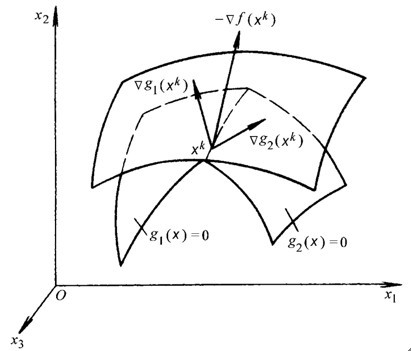
\includegraphics[width=0.5\textwidth]{KKT-geometry-1.jpg}
\end{FigureCenter}


注意我们上面推导过, 约束起作用时 $ g_{j}({x})=0 $, 所以此时约束在几何上应该是一簇\textbf{约束平面}.

我们假设在 $ {x}^{*} $ 取得极小值点, 若同时满足 $ g_{1}({x})=0 $ 和 $ g_{2}({x})=0 $, 则 $ {x}^{k} $ 一定在这两个平面的交线上, 且 $ -\nabla f\left({x}^{*}\right)=\sum_{j \in J} \mu_{j} \nabla g_{j}\left({x}^{*}\right) $, 即 $ -\nabla f\left({x}^{k}\right) 、 \nabla g_{1}\left({x}^{k}\right) $ 和 $ \nabla g_{2}\left({x}^{k}\right) $ 共面。

\begin{FigureCenter}{}
    \label{fig:kkt-2}
    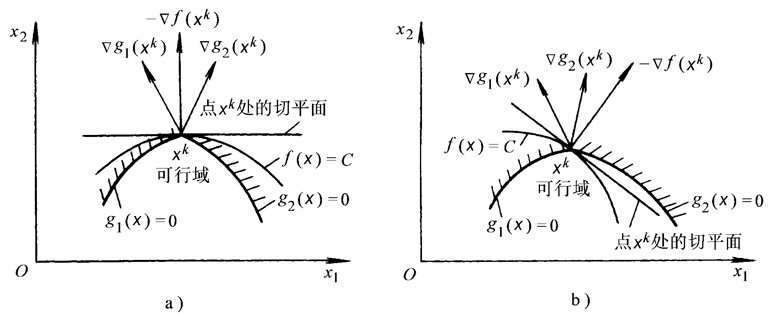
\includegraphics[width=\textwidth]{KKT-geometry-2.jpg}
\end{FigureCenter}

图\ref{fig:kkt-2}是在点 $ {x}^{k} $ 处沿 $ x_{1} O x_{2} $ 面的截面, 过点 $ {x}^{k} $ 作目标函数的负梯度 $ -\nabla f\left({x}^{k}\right) $, 它垂直于目标函数 的等值线 $ f({x})=C $ ,且指向目标函数 $ f({x}) $ 的最速减小方向。

\begin{corollary}
    一点的梯度与等值线相互垂直。
\end{corollary}

再作约束函数 $ g_{1}({x})=0 $ 和 $ g_{2}({x})=0 $ 的梯度 $ \nabla g_{1}\left({x}^{k}\right) $ 和 $ \nabla g_{2}\left({x}^{k}\right) $, 它们分别垂直 $ g_{1}({x})=0 $ 和 $ g_{2}({x})=0 $ 两曲面在 $ {x}^{k} $ 的切平面, 并形成一个雉形夹角区域。此时, 可能有 $ {a} 、 {b} $ 两种情形:

\begin{FigureCenter}{}
    \label{fig:kkt-3}
    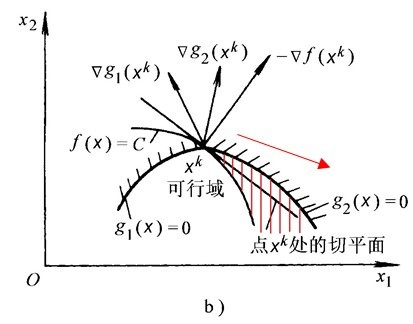
\includegraphics[width=0.5\textwidth]{KKT-geometry-3.jpg}
\end{FigureCenter}

我们先来看情形 ${b}$ :若3个向量的位置关系如\ref{fig:kkt-3}所示, 即 $-\nabla f$ 落在 $\nabla g_{1}$ 和 $\nabla g_{2}$ 所形成的锥角区外的 一侧。 此时, 作等值面 $f({x})=C$ 在点 ${x}^{k}$ 的切平面(它与 $-\nabla f\left({x}^{k}\right)$ 垂直), 我们发现:沿着与负 梯度 $-\nabla f$ 成锐角的方向移动(如下图红色箭头方向), 只要在红色区域取值, 目标函数 $f({x})$ 总 能减小。而红色区域是可行域 $(f({x})=C$, $C$取不同的常数能得到不同的等值线, 因此能取到红色 区域), 因此既可减小目标函数值, 又不破坏约束条件。 这说明 ${x}^{k}$ 仍可沿约束曲面移动而不破坏约 束条件, 且目标函数值还能够减小。所以 ${x}^{k}$ 不是稳定的最优点, 即不是局部极值点。

反过头来看情形a: $ -\nabla f $ 落在 $ \nabla g_{1} $ 和 $ \nabla g_{2} $ 形成的锥角内。 此时, 同样作 $ f({x})=C $ 在点 $ {x}^{k} $ 与 $ -\nabla f $ 垂直的切平面。 当从 $ {x}^{k} $ 出发沿着与负梯度 $ -\nabla f $ 成锐角的方向移动时, 虽然能使目标函数值减小, 但此时任何一点都不在可行区域内。 显然, 此时 $ {x}^{k} $ 就是局部最优点 $ {x}^{*} $, 再做任何移动都将破坏约 束条件, 故它是稳定点。

由于 $ -\nabla f\left({x}^{*}\right) $ 和 $ \nabla g_{1}\left({x}^{*}\right) 、 \nabla g_{2}\left({x}^{*}\right) $ 在一个平面内, 所以前者可看成是后两者的线性组合。 又由 上面的几何分析知, $ -\nabla f\left({x}^{*}\right) $ 在 $ \nabla g_{1}\left({x}^{*}\right) $ 和 $ \nabla g_{2}\left({x}^{*}\right) $ 的夹角之间, 所以线性组合的系数为正, 有
\begin{equation}
-\nabla f\left({x}^{*}\right)=\mu_{1} \nabla g_{1}\left({x}^{*}\right)+\mu_{2} \nabla g_{2}\left({x}^{*}\right), \text { 且 } \mu_{1}>0, \mu_{2}>0 \text {. }
\end{equation}
这就是 $ \mu_{j}>0 $ 的原因。 类似地, 当有多个不等式约束同时起作用时, 要求 $ -\nabla f\left({x}^{*}\right) $ 处于 $ \nabla g_{j}\left({x}^{*}\right) $ 形成的超角锥(高维图形, 我姑且称之为 “超” )之内。

\subsection{总结:同时包含等式和不等式约束的一般优化问题}

\begin{theorem}[同时包含等式和不等式约束的一般优化问题的KKT条件]
    \begin{equation}
\begin{array}{l}
\min f({x}) \\
\text { s.t. } g_{j}({x}) \leq 0(j=1,2, \cdots, m) \\
h_{k}({x})=0(k=1,2, \cdots, l)
\end{array}
\end{equation}
KKT条件 $ \left({x}^{*}\right. $ 是最优解的必要条件 $ ) $ 为
\begin{equation}
\left\{\begin{array}{l}
\frac{\partial f}{\partial x_{i}}+\sum_{j=1}^{m} \mu_{j} \frac{\partial g_{j}}{\partial x_{i}}+\sum_{k=1}^{l} \lambda_{k} \frac{\partial h_{k}}{\partial x_{i}}=0,(i=1,2, \ldots, n) \\
h_{k}({x})=0,(k=1,2, \cdots, l) \\
\mu_{j} g_{j}({x})=0,(j=1,2, \cdots, m) \\
\mu_{j} \geq 0
\end{array}\right.
\end{equation}
\end{theorem}

\begin{remark}
    对于等式约束的Lagrange乘子,并没有非负的要求。
\end{remark}

\begin{remark}
    以后求其极值点,不必再引入松弛变量,直接使用KKT条件判断。
\end{remark}


\section[Supplement Material: 凸优化、拉格朗日乘子法和KKT条件]{Supplement Material: 凸优化、拉格朗日乘子法和KKT条件\footnote{Cited from \url{https://zhuanlan.zhihu.com/p/59928816}.}}

\subsection{凸集的概念}

\begin{definition}[点、(直)线、线段]
    $ x_{1} \neq x_{2} $ 是 $ \mathbb{R}^{n} $ 中的两\term{点}, $ \theta \in \mathbb{R} $, 那么 $ y=x_{2}+\theta\left(x_{1}-x_{2}\right) $ 表示穿过两点的\term{线}.

    当 $ 0 \leqslant \theta \leqslant 1 $ 时, $ y $ 是 $ x_{1} $ 到 $ x_{2} $ 的\term{线段},$ y $ 也可以表示成 $ y=\theta x_{1}+(1-\theta) x_{2} $.
\end{definition}

\begin{definition}[仿射集]
    一个集合 $ C \subseteq \mathbb{R}^{n} $ 是\term{仿射集}如果其中任意两个不同的点的连线仍包含于 $ C $ .
\end{definition}

\begin{definition}[凸集]
    一个集合 $ C \subseteq \mathbb{R}^{n} $ 是凸集, 如果任意两点之间的线段仍包含于 $ C $ .即 $ \forall x_{1}, x_{2} \in C $, 任意 $ 0 \leqslant \theta \leqslant 1 $, 有 $ \theta x_{1}+(1-\theta) x_{2} \in C $ .
\end{definition}

\begin{theorem}
    两个凸集的交集仍是凸集。
\end{theorem}

\begin{definition}[凸函数]
    一个函数 $ f: \mathbb{R}^{n} \rightarrow \mathbb{R} $ 是\term{凸函数}如果定义域是凸集而且对任意定义域的 $ x, y, 0 \leqslant \theta \leqslant 1 $ 有
\begin{equation}
f(\theta x+(1-\theta) y) \leqslant \theta f(x)+(1-\theta) f(y)
\end{equation}
\end{definition}

二维时候的几何意义是, 如果两点的线段总位于函数曲线之上, 那么该函数是凸函数。

\begin{theorem}
    $ f $ 是凸的, 那么 $ -f $ 是 凹的。
\end{theorem}

\begin{theorem}
    
仿射函数既凸又凹。
\end{theorem}


\begin{theorem}[$ \alpha- $sublevel 集]
    给定凸函数 $ f$,则$\{x \in D(f): f(x) \leqslant \alpha\} $是一个凸集。
\end{theorem}

\begin{proof}
    对任意 $ x, y \in D(f) $ 使得 \begin{equation} f(x) \leqslant \alpha, f(y) \leqslant \alpha \end{equation}
    
    有 \begin{equation} f(\theta x+(1-\theta) y) \leqslant \theta f(x)+(1-\theta) f(y) \leqslant \theta \alpha+(1-\theta) \alpha \end{equation}
    
    也就是说如果 $ x, y $ 属于 $ \alpha- $ sublevel 集,那么二者之间的线段上的点也可以使得 $ f \leqslant \alpha , $ 即二者之间的线段也包含于 $ \alpha- $ sublevel 集。
\end{proof}

\subsection{凸优化}

\begin{definition}[优化问题]
    \term{优化问题}有如下形式:

    \begin{equation}
\begin{array}{ll}
\operatorname{minimize} & f_{0}(x) \\
\text { subject to } & f_{i}(x) \leqslant b_{i}, i=1, \ldots, m
\end{array}
\end{equation}

$ x=\left(x_{1}, \ldots, x_{n}\right) $ 是\term{优化变量}, 函数 $ f_{0}: \mathbb{R}^{n} \rightarrow \mathbb{R} $ 是\term{目标函数}, 函数 $ f_{i}: \mathbb{R}^{n} \rightarrow \mathbb{R} $ 是\term{约束函数}. $ b_{i} $ 是约束。使得 $ f_{0}(x) $ 在约束条件下最小的 $ x^{*} $ 叫做\term{最优点}, 或问题的\term{解}.
\end{definition}

\begin{definition}[凸优化]
    \term{凸优化}问题有如下形式:

    \begin{equation}
    \begin{array}{ll}
    \operatorname{minimize} & f(x) \\
    \text { subject to } & x \in C
    \end{array}
    \end{equation}
    
    $ f $ 是凸函数, $ C $ 是凸集。
\end{definition}

\begin{corollary}
    凸集可以表示成某些凸集的交集。
\end{corollary}

所以凸优化问题一般表示为

\begin{definition}[凸优化问题]
    \label{def:convex-problem}

    \begin{equation}
    \begin{array}{ll}
    \operatorname{minimize} & f(x) \\
    \text { subject to } & g_{i}(x) \leqslant 0, i=1, \ldots, m \\
    & h_{j}(x)=0, j=1, \ldots, p
    \end{array}
    \end{equation}

    其中 $ g_{i} $ 是\term{凸函数}, $ h_{j} $ 是\term{仿射函数}. 
\end{definition}

$ g_{i}(x) \leqslant 0 $叫做 \term{$ 0- $sublevel集}, 是凸集。

\begin{theorem}
    $ h_{j}(x)=0 $ 也是凸集。
\end{theorem}

\begin{proof}
    \begin{equation} h\left(\theta x_{1}+(1-\theta) x_{2}\right)=\theta h\left(x_{1}\right)+(1-\theta) h\left(x_{2}\right)=0 \end{equation}
\end{proof}

凸优化问题的特点是, \textbf{所有局部最优点都是全局最优点}.

\begin{definition}[二次规划]
    如果一个凸优化问题的 $ g_{i} $ 都是仿射函数, 且 $ f $ 是凸二次函数, 那么它叫做二次规划:
    \begin{equation}
    \begin{array}{ll}
    \operatorname{minimize} & \frac{1}{2} x^{\top} P x+c^{\top} x+d \\
    \text { subject to } & g_{i}(x) \leqslant 0, i=1, \ldots, m \\
    & h_{j}(x)=0, j=1, \ldots, p
    \end{array}
    \end{equation}

    其中 $ P $ 是一个对称半正定矩阵(使得 $ \left.\frac{1}{2} x^{\top} P x \geqslant 0\right) $ .
\end{definition}



\subsection{拉格朗日对偶性}

\begin{theorem}
    对于没有限制的凸函数, 最优点 $ x^{*} $ 一定满足 $ \nabla_{x} f\left(x^{*}\right)=0 $.
\end{theorem}

然而对于有限制条件的凸优化问题却不是这样。拉格朗日对偶性可以将有限制的凸优化问题转化为没有限制的问题, 来求解凸优化问题。

\begin{definition}[拉格朗日函数]
    给定一个凸优化问题, 拉格朗日算子是一个函数 $ \mathcal{L}: \mathbb{R}^{n} \times \mathbb{R}^{m} \times \mathbb{R}^{p} \rightarrow \mathbb{R} $, 定义为:
    \begin{equation}
    \mathcal{L}(x, \alpha, \beta)=f(x)+\sum_{i=1}^{m} \alpha_{i} g_{i}(x)+\sum_{i=1}^{p} \beta_{i} h_{i}(x)
    \end{equation}

    $ x \in \mathbb{R}^{n} $ 叫做\term{主变量(primal variable)}. $ \alpha \in \mathbb{R}^{m}, \beta \in \mathbb{R}^{p} $ 统称对偶变量或拉格朗日乘子。
\end{definition}

\begin{theorem}
    总存在一个拉格朗日乘子, 使得没有限制的拉格朗日算子相对于 $ x $ 的最小值, 等于原凸优化问题的最优值
\end{theorem}

后文会证明。

\subsubsection{主问题}

为了说明拉格朗日算子和原凸优化问题的关系,需要引入主问题和对偶问题。

考虑优化问题:

\begin{problem}
    \label{pbl:primal}
    \begin{equation}
\min _{x}\left[\max _{\alpha, \beta, \alpha_{i} \geqslant 0} \mathcal{L}(x, \alpha, \beta)\right]=\min _{x} \theta_{\mathcal{P}}(x)
\end{equation}

括号内的 $ \theta_{\mathcal{P}}: \mathbb{R}^{n} \rightarrow \mathbb{R} $ 叫做\term{主目标(primal objective)}, 等号右边的没有限制的最小化问题叫做\term{主问题(primal problem)}. 用 $ x^{*} $ 表示\term{主问题的解},$ p^{*}=\theta_{\mathcal{P}}\left(x^{*}\right) $ 表示\term{主目标的最优值}.
\end{problem}

\begin{definition}[primal feasible]
    $ x $ 是\term{主可行的(primal feasible)}如果 $ g_{i}(x) \leqslant 0, h_{j}(x)=0 $ .
\end{definition}


\begin{equation}
\begin{aligned}
\theta_{\mathcal{P}}(x) &=\max _{\alpha, \beta, \alpha_{i} \geqslant 0} \mathcal{L}(x, \alpha, \beta) \\
&=\max _{\alpha, \beta, \alpha_{i} \geqslant 0}\left[f(x)+\sum_{i=1}^{m} \alpha_{i} g_{i}(x)+\sum_{i=1}^{p} \beta_{i} h_{i}(x)\right] \\
&=f(x)+\max _{\alpha, \beta, \alpha_{i} \geqslant 0}\left[\sum_{i=1}^{m} \alpha_{i} g_{i}(x)+\sum_{i=1}^{p} \beta_{i} h_{i}(x)\right]
\end{aligned}
\end{equation}

观察最后一个式子:

\begin{itemize}
    \item 如果任何一个 $ g_{i}(x)>0 $, 那么最大化 $ \theta_{\mathcal{P}}(x) $ 只需要将相应的 $ \alpha_{i} $ 设置为无限大。
    \item 如果 $ g_{i}(x) \leqslant 0 $, 因为 $ \alpha_{i} \geqslant 0 $, 所以 $ \theta_{\mathcal{P}}(x) $ 最大时, 必然有 $ \alpha_{i}=0 $ .
\end{itemize}

相似地:

\begin{itemize}
    \item 如果 $ h_{i} \neq 0 $, 那么最大化 $ \theta_{\mathcal{P}}(x) $ 只需要将相应的 $ \beta_{i} $ 设置为 $ h_{i}(x) $ 的相同符号且绝对值无限大。
    \item 如果 $ h_{i}(x)=0 $, 那么 $ \sum_{i=1}^{p} \beta_{i} h_{i}(x) $ 项的最大值为0 .
\end{itemize}

综上, 有
\begin{equation}
\theta_{\mathcal{P}}(x)=\left\{\begin{array}{ll}
f(x)+0 & x \text { 为主可行的 } \\
f(x)+\infty & x \text { 不是主可行的 }
\end{array}\right.
\end{equation}
因此当 $ x $ 主可行时, 主问题\ref{pbl:primal}的最优值等于原凸优化问题\ref{def:convex-problem}的最优值。

\subsubsection{对偶问题}

\begin{definition}[对偶问题]
    对调主问题的最大最小操作:
\begin{equation}
\max _{\alpha, \beta, \alpha \geqslant 0}\left[\min _{x} \mathcal{L}(x, \alpha, \beta)\right]=\max _{\alpha, \beta, \alpha \geqslant 0} \theta_{\mathcal{D}}(\alpha, \beta)
\end{equation}

$ \theta_{\mathcal{D}}(\alpha, \beta): \mathbb{R}^{m} \times \mathbb{R}^{p} \rightarrow \mathbb{R} $ 是\term{对偶目标(dual objective)},等号右边的有限制的最大化问题叫做\term{对偶问题}. 用 $ \left(\alpha^{*}, \beta^{*}\right) $ 表示\term{对偶问题的解}, $ d^{*}=\theta_{\mathcal{D}}\left(\alpha^{*}, \beta^{*}\right) $ 表示\term{对偶目标的最优值}.
\end{definition}

\begin{definition}[对偶可行]
    如果 $ \alpha_{i}(x) \geqslant 0 $ ,$ (\alpha, \beta) $ 是对偶可行的。
\end{definition}


\begin{theorem}
    如果 $ (\alpha, \beta) $ 是对偶可行的,那么 $ \theta_{\mathcal{D}}(\alpha, \beta) \leqslant p^{*} $.
\end{theorem}

\begin{proof}
    \begin{equation} \begin{aligned} \theta_{\mathcal{D}}(\alpha, \beta) &=\min _{x} \mathcal{L}(x, \alpha, \beta) \\ & \leqslant \mathcal{L}\left(x^{*}, \alpha, \beta\right) \\ &=f\left(x^{*}\right)+\sum_{i=1}^{m} \alpha_{i} g_{i}\left(x^{*}\right)+\sum_{i=1}^{p} \beta_{i} h_{i}\left(x^{*}\right) \\ & \leqslant f\left(x^{*}\right)=p^{*} \end{aligned} \end{equation}
\end{proof}

\begin{theorem}[弱对偶性]
    对任意主问题和对偶问题,有 $ d^{*} \leqslant p^{*} $.
\end{theorem}

\begin{theorem}[强对偶性]
    对任意主问题和对偶问题, 如果满足某个条件(constraint qualifications), 那 么 $ d^{*}=p^{*} $ .最常用的constraint qualification是Slater's condition: 所有的不等式限制都严格满 足 (即 $ g_{i}(x)<0 $ ) .
\end{theorem}

\begin{theorem}[Slater 条件]
    设定义在 $ \mathcal{D} $ 上的函数 $ f_{i}(\cdot), i=1,2, \cdots, n $ 为凸函数, $ g_{j}(\cdot), j=1,2, \cdots, m $ 为 仿射函数, 考虑凸优化问题

    \begin{equation}
    \min _{{x}} f_{0}({x}), \quad \text { s.t. } f_{i}({x}) \leq 0, g_{i}({x}) \leq 0
    \end{equation}

    如果存在点 $ {x} \in $ relint $ \mathcal{D} $ (即 $ \mathcal{D} $ 的相对内点), 则强对偶性成立。
\end{theorem}

实践中, 几乎所有的凸优化问题都满足某种constraint qualification, 所以 主问题和对偶问题有相同的最优值。

\begin{theorem}[互补松弛性 (complementary slackness, KKT complementarity)]
    如果强对偶性满足, 那么 $ \alpha_{i}^{*} g\left(x_{i}^{*}\right)=0, i=1, \ldots, m $
    
\end{theorem}

\begin{proof}
    \begin{equation}
    \begin{aligned}
    p^{*}=d^{*}=\theta_{\mathcal{D}}\left(\alpha^{*}, \beta^{*}\right) &=\min _{x} \mathcal{L}\left(x, \alpha^{*}, \beta^{*}\right) \\
    & \leqslant \mathcal{L}\left(x^{*}, \alpha^{*}, \beta^{*}\right) \\
    &=f\left(x^{*}\right)+\sum_{i=1}^{m} \alpha_{i}^{*} g_{i}\left(x^{*}\right)+\sum_{i=1}^{p} \beta_{i}^{*} h_{i}\left(x^{*}\right) \\
    & \leqslant f\left(x^{*}\right)=p^{*}
    \end{aligned}
    \end{equation}

    因为第一个和最后一个表达式相等, 所以中间所有的小于等于号都是等号, 有 \begin{equation} \sum_{i=1}^{m} \alpha_{i}^{*} g_{i}\left(x^{*}\right)+\sum_{i=1}^{p} \beta_{i}^{*} h_{i}\left(x^{*}\right)=0 \end{equation}

    因为 $ \alpha_{i}^{*} \geqslant 0 , h_{i}\left(x^{*}\right)=0 $, 所以 $ \alpha_{i}^{*} $ 和 $ g_{i}\left(x^{*}\right) $ 至少有一个是 0 .
\end{proof}

\begin{theorem}
    设 $ x^{*} \in \mathbb{R}^{n}, \alpha^{*} \in \mathbb{R}^{m}, \beta^{*} \in \mathbb{R}^{p} $, 下列条件为 $ {KKT} $ 条件:

    \begin{enumerate}
        \item (主可行) \begin{equation} g_{i}\left(x^{*}\right) \leqslant 0, i=1, \ldots, m, h_{j}\left(x^{*}\right)=0, j=1, \ldots, p \end{equation}
        \item (对偶可行) \begin{equation} \alpha_{i}^{*} \geqslant 0, i=1, \ldots, m \end{equation}
        \item (互补松弛性) \begin{equation} \alpha_{i}^{*} g\left(x_{i}^{*}\right)=0, i=1, \ldots, m \end{equation}
        \item (Lagrangian Stationary) \begin{equation} \nabla_{x} \mathcal{L}\left(x^{*}, \alpha^{*}, \beta^{*}\right)=0 \end{equation}
    \end{enumerate}

\end{theorem}

\begin{theorem}
    对于凸优化问题, 有:

$ x^{*} $ 原始最优, $ \left(\alpha^{*}, \beta^{*}\right) $ 对偶最优,且有\begin{equation} 强对偶性 \Leftrightarrow  满足  K K T  条件\end{equation}
\end{theorem}

\subsection{总结}


给定一个\term{凸优化}问题, \term{拉格朗日算子}将凸优化问题的目标函数和限制考虑进一个函数中, 在拉格朗日算子基础上可以定义\term{主问题}和\term{对偶问题}.

\term{主问题}是先调整 $ (\alpha, \beta) $ 使拉格朗日算子最大(变为主目标), 再调整 $ x $ 使主目标最小。 $ x $ 主可行时, 主目标等于原凸优化问题的目标函数, 主目标的最小值等于原凸优化问题的最小值。

\term{对偶问题}是先调整 $ x $ 使拉格朗日算子最小(变为对偶目标, 因为拉格朗日算子是关于 $ x $ 的没有限制 的凸函数, 所以变为对偶目标时其对 $ x $ 的偏导数为 0 ), 再调整使对偶目标最大。 $ (\alpha, \beta) $ 对偶可行 时, 对偶目标小于等于主目标的最小值。

\term{弱对偶性}指对偶目标的最大值小于等于主目标的最小值。强对偶性指对偶目标的最大值等于主目标的最小值。

\begin{equation}对偶目标的最大值=主目标的最小值=原凸优化问题的最小值 \Leftrightarrow^{当且仅当}满足KKT条件\end{equation}

因此,当对偶问题比原凸优化问题容易求解时,可以通过求解对偶问题来解原凸优化问题。


\section[Supplementary Material: KKT Conditions, Linear Programming and Nonlinear Programming]{Supplementary Material: KKT Conditions, Linear Programming and Nonlinear Programming \footnote{Written by Christopher Griffine. (\href{http://www.personal.psu.edu/cxg286/LinearProgramming.html}{Linear Programming})}}



\subsection{Karush-Kuhn-Tucker Theorem(s)}

\begin{theorem} Let $z : \mathbb{R}^n \rightarrow \mathbb{R}$ be a differentiable objective function, $g_i:\mathbb{R}^n \rightarrow \mathbb{R}$ be differentiable constraint functions for $i = 1,\dots,m$ and $h_j:\mathbb{R}^n \rightarrow \mathbb{R}$ be differentiable constraint functions for $j=1,\dots,l$. If ${x}^* \in \mathbb{R}^n$ is an optimal point satisfying an appropriate regularity condition for the following optimization problem:

\begin{equation}
P\left\{
\begin{aligned}
\max\;\;& z(x_1,\dots,x_n)\\
s.t.\;\;& g_1(x_1,\dots,x_n) \leq 0\\
& \hspace*{0.5in}\vdots\\
& g_m(x_1,\dots,x_n) \leq 0\\
& h_1(x_1,\dots,x_n) = 0\\
&\hspace*{0.5in}\vdots\\
&h_l(x_1,\dots,x_n) = 0
\end{aligned}
\right.
\end{equation}

then there exists $\lambda_1,\dots,\lambda_m \in \mathbb{R}$ and $\mu_1,\dots\mu_l \in \mathbb{R}$ so that:

\begin{gather*}
\text{Primal Feasibility}: \left\{
\begin{aligned}
g_i({x}^*) \leq 0 \quad \text{for $i = 1,\dots,m$}\\
h_j({x}^*) = 0 \quad \text{for $j = 1,\dots,l$}
\end{aligned}
\right.\\
\text{Dual Feasibility}:\left\{
\begin{aligned}
\nabla z({x}^*) - \sum_{i = 1}^m\lambda_i\nabla g_i({x}^*) - \sum_{j = 1}^{l}\mu_j\nabla h_j({x}^*) = {0}\\
\lambda_i \geq 0 \quad \text{for $i=1,\dots,m$}\\
\mu_j \in \mathbb{R} \quad \text{for $j = 1,\dots,l$}
\end{aligned}
\right.\\
\text{Complementary Slackness}:\left\{
\begin{aligned}
\lambda_ig_i({x}^*) = 0 \quad \text{for $i = 1,\dots,m$}
\end{aligned}
\right.
\end{gather*}
\label{thm:KKT7}
\end{theorem}

\begin{theorem} Let $z : \mathbb{R}^n \rightarrow \mathbb{R}$ be a differentiable concave (凹) function, $g_i:\mathbb{R}^n \rightarrow \mathbb{R}$ be differentiable convex functions for $i = 1,\dots,m$ and $h_j:\mathbb{R}^n \rightarrow \mathbb{R}$ be affine functions for $j=1,\dots,l$. Suppose there are $\lambda_1,\dots,\lambda_m \in \mathbb{R}$ and $\mu_1,\dots\mu_l \in \mathbb{R}$ so that:

\begin{gather*}
\text{Primal Feasibility}: \left\{
\begin{aligned}
g_i({x}^*) \leq 0 \quad \text{for $i = 1,\dots,m$}\\
h_j({x}^*) = 0 \quad \text{for $j = 1,\dots,l$}
\end{aligned}
\right.\\
\text{Dual Feasibility}:\left\{
\begin{aligned}
\nabla z({x}^*) - \sum_{i = 1}^m\lambda_i\nabla g_i({x}^*) - \sum_{j = 1}^{l}\mu_j\nabla h_j({x}^*) = {0}\\
\lambda_i \geq 0 \quad \text{for $i=1,\dots,m$}\\
\mu_j \in \mathbb{R} \quad \text{for $j = 1,\dots,l$}
\end{aligned}
\right.\\
\text{Complementary Slackness}:\left\{
\begin{aligned}
\lambda_ig_i({x}^*) = 0 \quad \text{for $i = 1,\dots,m$}
\end{aligned}
\right.
\end{gather*}

then ${x}^*$ is a global maximizer for 
\begin{equation}
P\left\{
\begin{aligned}
\max\;\;& z(x_1,\dots,x_n)\\
s.t.\;\;& g_1(x_1,\dots,x_n) \leq 0\\
& \hspace*{0.5in}\vdots\\
& g_m(x_1,\dots,x_n) \leq 0\\
& h_1(x_1,\dots,x_n) = 0\\
&\hspace*{0.5in}\vdots\\
&h_l(x_1,\dots,x_n) = 0
\end{aligned}
\right.
\end{equation}
\label{thm:KKT8}
\end{theorem}

The values $\lambda_1,\dots,\lambda_m$ and $\mu_1,\dots,\mu_l$ are sometimes called \term{Lagrange multipliers} and sometimes called \term{dual variables}. Primal Feasibility, Dual Feasibility and Complementary Slackness are called the \term{Karush-Kuhn-Tucker} (KKT) conditions.

\begin{remark} The regularity condition mentioned in Theorem \ref{thm:KKT7} is sometimes called a \term{constraint qualification}. A common one is that the gradients of the binding constraints are all linearly independent at ${x}^*$. There are many variations of constraint qualifications. We will not deal with these in these notes. 
    
    Suffice it to say, all the problems we consider will automatically satisfy a constraint qualification, meaning the KKT theorem holds.
\end{remark}

\begin{remark} Theorem \ref{thm:KKT7} holds as a necessary condition even if $z({x})$ is not concave or the functions $g_i({x})$ ($i=1,\dots,m$) are not convex or the functions $h_j({x})$ ($j=1,\dots,l$) are not linear. In this case though, the fact that a triple: $({x},\boldsymbol{\lambda}, \boldsymbol{\mu}) \in \mathbb{R}^{n} \times \mathbb{R}^m \times \mathbb{R}^l$ does not ensure that this is an optimal solution for Problem $P$.
\end{remark}

Looking more closely at the dual feasibility conditions, we see something interesting. Suppose that there are \term{no} equality constraints (i.e., not constraints of the form $h_j({x}) = 0$). Then the statements:

\begin{equation}
\begin{aligned}
\nabla z({x}^*) - \sum_{i = 1}^m\lambda_i \nabla g_i({x}^*) - \sum_{j = 1}^{l}\mu_j \nabla h_j({x}^*) & = {0}\\
\lambda_i &\geq 0 \quad \text{for $i=1,\dots,m$}
\end{aligned}
\end{equation}

imply that:

\begin{equation}
\begin{aligned}
\nabla z({x}^*) &= \sum_{i = 1}^m\lambda_i \nabla g_i({x}^*)\\
\lambda_i &\geq 0 \quad \text{for $i=1,\dots,m$}
\end{aligned}
\end{equation}

Specifically, this says that the \term{gradient of $z$ at ${x}^*$ is a positive combination of the gradients of the constraints at ${x}^*$.} But more importantly, since we also have \term{complementary slackness}, we know that if ${g}_i({x}^*) \neq 0$, then $\lambda_i = 0$ because $\lambda_i g_i({x}^*) = 0$ for $i = 1,\dots,m$. Thus, what dual feasibility is really saying is that \term{gradient of $z$ at ${x}^*$ is a positive combination of the  gradients of the \textbf{binding} constraints at ${x}^*$.} Remember, a constraint is binding if $g_i({x}^*) = 0$, in which case $\lambda_i \geq 0$.


\begin{remark} Continuing from the previous remark, in the general case when we have some equality constraints, then dual feasibility says:
\begin{equation}
\begin{aligned}
\nabla z({x}^*) &= \sum_{i = 1}^m\lambda_i \nabla g_i({x}^*) + \sum_{j = 1}^{l}\mu_j \nabla h_j({x}^*)\\
\lambda_i &\geq 0 \quad \text{for $i=1,\dots,m$}\\
\mu_j &\in \mathbb{R}\quad \text{for $j=1,\dots,l$}
\end{aligned}
\end{equation}
Since equality constraints are \term{always binding} this says that the \term{gradient of $z$ at ${x}^*$ is a linear combination of the  gradients of the \textbf{binding} constraints at ${x}^*$.} 
\end{remark}

\subsection{Linear Programming and KKT Conditions - An Example}
Consider the following linear programming problem:
\begin{equation}
P \left \{
\begin{aligned}
\max \;\; & x_1 + x_2  \\ 
s.t. & x_1 + 2x_2 \leq 4\\
& 2x_1 + x_2 \leq 6\\
& x_1, x_2 \geq 0
\end{aligned} \right.
\end{equation}
Assuming I didn't know how to solve this problem using the Simplex method, I could look at Theorem \ref{thm:KKT8} and remark that the constraints and objective are all concave (and convex) since they are linear. Therefore, it suffices to find a KKT point and this point must be optimal.
We can re-write Problem $P$ in the form of Theorem \ref{thm:KKT7} as:
\begin{equation}
P \left \{
\begin{aligned}
\max \;\; & z(x_1,x_2) \equiv x_1 + x_2  \\ 
s.t. & g_1(x_1,x_2) \equiv x_1 + 2x_2 -4 \leq 0\\
& g_2(x_1,x_2) \equiv 2x_1 + x_2 - 6\leq 0\\
& g_3(x_1,x_2) \equiv -x_1 \leq 0\\
& g_4(x_1,x_2) \equiv -x_2 \leq 0
\end{aligned} \right.
\end{equation}

To write the KKT conditions, observe the following:
\begin{equation}
\nabla z = \begin{bmatrix}1\\1\end{bmatrix} \quad \quad \nabla g_1 = \begin{bmatrix}1\\2\end{bmatrix}
\quad\quad \nabla g_2 = \begin{bmatrix}2\\1\end{bmatrix} \quad \quad 
\nabla g_3 = \begin{bmatrix}-1\\0\end{bmatrix} \quad \quad \nabla g_4 = \begin{bmatrix}0\\-1\end{bmatrix}
\end{equation}
We can now write the KKT conditions for this problem as:
\begin{gather*}
\text{Primal Feasibility}: \left\{
\begin{aligned}
x_1 + 2x_2 &\leq 4\\
2x_1 + x_2 &\leq 6\\
x_1, x_2 &\geq 0
\end{aligned}
\right.\\
\text{Dual Feasibility}:\left\{
\begin{aligned}
\begin{bmatrix}1\\1\end{bmatrix} - \lambda_1\begin{bmatrix}1\\2\end{bmatrix} - 
\lambda_2\begin{bmatrix}2\\1\end{bmatrix} -\lambda_3\begin{bmatrix}-1\\0\end{bmatrix} - 
\lambda_4\begin{bmatrix}0\\-1\end{bmatrix} &= \begin{bmatrix}0\\0\end{bmatrix}\\
\lambda_1,\lambda_2,\lambda_3,\lambda_4 & \geq 0
\end{aligned}
\right.\\
\text{Complementary Slackness}:\left\{
\begin{aligned}
\lambda_1(x_1 + 2x_2 -4) &= 0\\
\lambda_2(2x_1 + x_2 - 6) &= 0\\
\lambda_3(-x_1) &= 0\\
\lambda_4(-x_2) &= 0
\end{aligned}
\right.
\end{gather*}
Consider Dual Feasibility for a moment. I can expand the matrices to obtain a system of equations:
\begin{equation}
\begin{aligned}
1 - \lambda_1 - 2\lambda_2 + \lambda_3 & = 0\\
1 - 2\lambda_1 - \lambda_2 + \lambda_4 & = 0\\
\lambda_1,\lambda_2,\lambda_3,\lambda_4 & \geq 0
\end{aligned}
\end{equation}
Or:
\begin{equation}
\begin{aligned}
\lambda_1 + 2\lambda_2 - \lambda_3 &= 1\\
2\lambda_1 + \lambda_2 - \lambda_4 &= 1\\
\lambda_1,\lambda_2,\lambda_3,\lambda_4 & \geq 0
\end{aligned}
\end{equation}
Since $\lambda_3, \lambda_4 \geq 0$, they act like \term{surplus variables} and we can write the Dual Feasibility as:
\begin{equation}
\left\{
\begin{aligned}
\lambda_1 + 2\lambda_2 &\geq  1\\
2\lambda_1 + \lambda_2 &\geq 1\\
\lambda_1,\lambda_2& \geq 0
\end{aligned}\right.
\label{eqn:Lambda}
\end{equation}
\begin{remark} It would now suffice to find values for $x_1$, $x_2$, $\lambda_1$, $\lambda_2$, $\lambda_3$, and $\lambda_4$ the satisfy the KKT conditions and we could solve the linear programming problem $P$.
\end{remark}

We can show that the optimal point for this problem is $x = \tfrac{8}{3}$ and $y = \tfrac{2}{3}$ using a graphical method. Figure \ref{fig:KKTLP-1} shows the feasible region of the problem as well as the level curves of the objective function (curves for which $x_1 + x_2 = k$, where $k$ is a fixed constant). The value $k$ increases going left to right and bottom to top, so the optimal solution must occur at the intersection of the lines $x_1 + 2 x_2 = 4$ and $2x_1 + x_2 = 6$. You can compare the value of the objective at the proposed optimal point $x = \tfrac{8}{3}$ and $y = \tfrac{2}{3}$ to the value of the objective at the other extreme points. For example, at the extreme point $x = 3$, $y = 0$, we see the value of the objective is only $3$, as compared to $\tfrac{10}{3}$ at the point of optimality.


\begin{FigureCenter}{The feasible region for the example linear programming problem illustrating level curves of the objective.}
    \label{fig:KKTLP-1}
    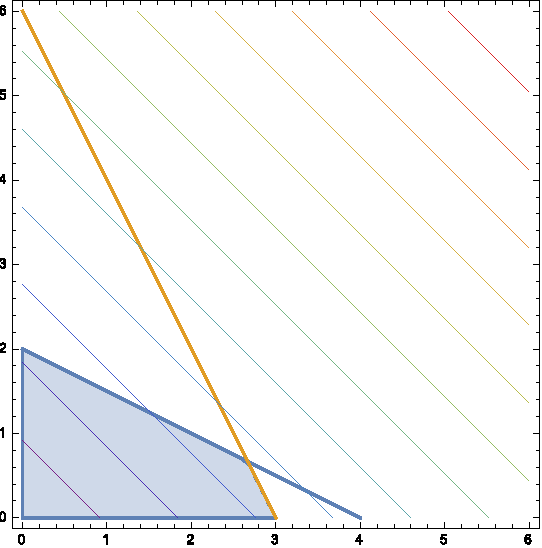
\includegraphics[width=0.4\textwidth]{imported_figures/KKTLP-1-eps-converted-to.pdf}
\end{FigureCenter}

\begin{FigureCenter}{The gradients of the objective function and the binding constraints at optimality and their geometric relation are illustrated}
    \label{fig:KKTLP-2}
    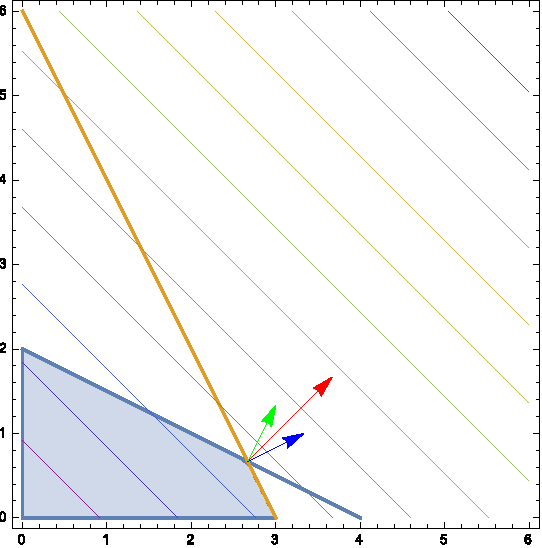
\includegraphics[width=0.4\textwidth]{imported_figures/KKTLP-2-eps-converted-to.pdf}
\end{FigureCenter}


We can now see that for the KKT conditions to hold, we must have $\lambda_3 = \lambda_4 = 0$ because $x_1 > 0$ and $x_2 > 0$ at optimality and complementary slackness requires that: $\lambda_3(-x_1) = 0$ and $\lambda_4(-x_2) = 0$ at optimality. This leaves $\lambda_1$ and $\lambda_2$. We know these must satisfy the equations in Expression \ref{eqn:Lambda}. Therefore, we see that when $\lambda_1 = \lambda_2 = \tfrac{1}{3}$, Expression 2 is satisfied. Thus: we have written:
\begin{equation}
\begin{bmatrix}1\\1\end{bmatrix} = \frac{1}{3}\begin{bmatrix}1\\2\end{bmatrix} - 
\frac{1}{3}\begin{bmatrix}2\\1\end{bmatrix}
\end{equation}
That is, we have expressed the gradient of the objective function ($\nabla z$) as a positive combination of the gradients of the \term{binding} constraints ($\nabla g_1$ and $\nabla g_2$). This is shown in Figure \ref{fig:KKTLP-2}, in which we see the gradient of the objective function (red) inside the (cone of) the gradients of the binding constraints (blue and green).

\subsection{The Dual KKT Conditions}
Recall that if we are given a linear programming problem of the form:
\begin{equation}
P\left\{
\begin{aligned}
\max\;\; & {c}^T{x}\\
s.t.\;\; & {A}{x} \leq {b}\\
& {x} \geq 0
\end{aligned}\right.
\end{equation}

Then the dual problem for Problem $P$ is:
\begin{equation}
D\left\{
\begin{aligned}
\min\;\; & {w}{b}\\
s.t.\;\; & {w}{A} \geq {c}^T\\
& {w} \geq {0}
\end{aligned}\right.
\end{equation}
Here we assume that ${w}$ is a \term{row} vector (unlike our usual assumption that all vectors are column vectors). In our example problem, we have:
\begin{equation}
{A} = \begin{bmatrix}1 & 2\\2 & 1\end{bmatrix} \quad \quad {c} = \begin{bmatrix}1\\1\end{bmatrix} \quad \quad {b} = \begin{bmatrix}4\\6\end{bmatrix}
\end{equation}
Let us write:
\begin{equation}
{w} = \begin{bmatrix} \lambda_1 & \lambda_2 \end{bmatrix}
\end{equation}
Then we can write the dual problem as:
\begin{equation}
D\left\{
\begin{aligned}
\min \;\; & \begin{bmatrix} \lambda_1 & \lambda_2 \end{bmatrix} \begin{bmatrix}4\\6\end{bmatrix} \\
& \begin{bmatrix} \lambda_1 & \lambda_2 \end{bmatrix} \begin{bmatrix}1 & 2\\2 & 1\end{bmatrix} \geq \begin{bmatrix}1 & 1\end{bmatrix}\\
& \lambda_1, \lambda_2 \geq 0
\end{aligned}
\right.
\end{equation}
This can be rewritten more concretely as:
\begin{equation}
D\left\{
\begin{aligned}
\min \;\; & 4\lambda_1 + 6\lambda_2\\
&\lambda_1 + 2\lambda_2 \geq 1\\
&2\lambda_1 + \lambda_2 \geq 1\\
& \lambda_1, \lambda_2 \geq 0
\end{aligned}
\right.
\end{equation}
Immediately we see a connection. The constraints of this problem look just like the simplified dual feasibility constraints. In fact, if we add surplus variables $\lambda_3, \lambda_4 \geq 0$, we see they match exactly and the problem in standard form is:
\begin{equation}
D\left\{
\begin{aligned}
\min \;\; & 4\lambda_1 + 6\lambda_2\\
&\lambda_1 + 2\lambda_2 - \lambda_3 = 1\\
&2\lambda_1 + \lambda_2 -\lambda_4 =1\\
& \lambda_1, \lambda_2,\lambda_3, \lambda_4 \geq 0
\end{aligned}
\right.
\end{equation}
We can complete our exploration of the relationship between these two problems by constructing the KKT conditions for the dual problem. First, re-write the dual as:
\begin{equation}
\begin{aligned}
\max\;\; & -4\lambda_1 - 6\lambda_2 \\
s.t. & -\lambda_1 - 2\lambda_2 + 1\leq 0\\
& -2\lambda_1 - \lambda_2 + 1\leq 0\\
& -\lambda_1 \leq 0\\
& -\lambda_2 \leq 0
\end{aligned}
\end{equation}
As before, we can write down the KKT conditions:

$$\text{Primal Feasibility}: \left\{
\begin{aligned}
\lambda_1 + 2\lambda_2 &\geq 1\\
2\lambda_1 + \lambda_2 &\geq 1\\
\lambda_1, \lambda_2 & \geq 1
\end{aligned}
\right.$$


$$\text{Dual Feasibility}:\left\{
\begin{aligned}
\begin{bmatrix}-4\\-6\end{bmatrix} - x_1\begin{bmatrix}-1\\-2\end{bmatrix} - 
x_2\begin{bmatrix}-2\\-1\end{bmatrix} -s_1\begin{bmatrix}-1\\0\end{bmatrix} - 
s_2\begin{bmatrix}0\\-1\end{bmatrix} &= \begin{bmatrix}0\\0\end{bmatrix}\\
x_1,x_2,s_1,s_2 & \geq 0
\end{aligned}
\right.$$

$$\text{Complementary Slackness}:\left\{
    \begin{aligned}
    x_1(-\lambda_1 - 2\lambda_2 + 1) &= 0\\
    x_2(-2\lambda_1 - \lambda_2 + 1) &= 0\\
    s_1(-\lambda_1) &= 0\\
    s_2(-\lambda_2) &= 0
    \end{aligned}
    \right.$$

Again, we can re-write the dual feasibility conditions (for which we have intentionally chosen specific dual variable names) and see they become:
\begin{equation}
\begin{aligned}
x_1 + 2x_2 + s_1 &= 4\\
2x_1 + x_2 + s_2 & =6\\
x_1,x_2, s_1, s_2 &\geq 0
\end{aligned}
\end{equation}
Since $s_1, s_2 \geq 0$, they act like \term{slack variables} and thus we have:
\begin{equation}
\begin{aligned}
x_1 + 2x_2 &\leq  4\\
2x_1 + x_2 &\leq 6\\
x_1,x_2&\geq 0
\end{aligned}
\end{equation}
and we've recovered the constraints from the original primal problem as the dual feasibility conditions of the KKT conditions for the dual optimization problem. We can go further. Note:
\begin{equation}
    \begin{aligned}
        -s_1 &= x_1 + 2x_2 - 4= -g_1(x_1,x_2)\\
-s_2 &= 2x_1 + x_2 -6 = -g_2(x_1,x_2)
    \end{aligned}
\end{equation}

while from our earlier observations about the surplus variables $\lambda_3$ and $\lambda_4$ we know:
\begin{equation}
    \begin{aligned}
        \lambda_3 &= -\lambda_1 - 2\lambda_2 + 1\\
    -\lambda_4 &= -2\lambda_1 - \lambda_2 + 1
    \end{aligned}
\end{equation}
Thus, complementary slackness from the primal problem is:
\begin{equation}
\begin{aligned}
    \lambda_3(-x_1) &= 0 \iff \lambda_3(x_1) =0  \iff 
	x_1(\lambda_1 + 2\lambda_2 - 1) = 0\\
\lambda_4(-x_2) &= 0 \iff \lambda_4(x_2) =0 \iff x_2(-2\lambda_1 - \lambda_2 + 1) = 0
\end{aligned}
\end{equation}
Likewise:
\begin{equation}
    \begin{aligned}
        \lambda_1(x_1 + 2x_2 - 4) &=0 \iff \lambda_1(-s_1) = 0 \iff s_1(-\lambda_1) = 0\\
\lambda_2(2x_1 + x_2 - 6) &=0 \iff \lambda_2(-s_2) = 0 \iff s_2(-\lambda_2) = 0
    \end{aligned}
\end{equation}
Thus, the complementary slackness conditions of the primal problem are identical to the complementary slackness conditions of the dual problem. This fact is true for linear programming problems in general.

\begin{remark} For an arbitrary linear programming problem and its dual, the KKT conditions for the primal and dual problems are \textbf{equivalent}, but the dual feasibility conditions for the primal problem are identical to the primal feasibility conditions for the dual problem and vice-versa. \term{Thus, two linear programming problems are dual to each other if and only if they share KKT conditions with the primal and dual feasibility conditions swapped.}
\end{remark}

\begin{remark} We will use these results on KKT conditions and linear programs to discuss the solution (i.e., Nash equilibria) of zero-sum games via linear programming. We will then generalize these results to derive a quadratic programming problem whose optimal solutions will yield Nash equilibria. 
\end{remark}

\subsection{An Example from Nonlinear Programming}
Let's recall a simple optimization problem from differential calculus (Math 140): Goats are an environmentally friendly and inexpensive way to control a lawn when there are lots of rocks or lots of hills. (Seriously, both Google and some U.S. Navy bases use goats on rocky hills instead of paying lawn mowers!) 

Suppose I wish to build a pen to keep some goats. I have 100 meters of fencing and I wish to build the pen in a rectangle with the largest possible area. How long should the sides of the rectangle be? In this case, making the pen \term{better} means making it have the largest possible area.

The problem is illustrated in Figure \ref{fig:GoatPen}.
\begin{figure}[htbp]
\centering
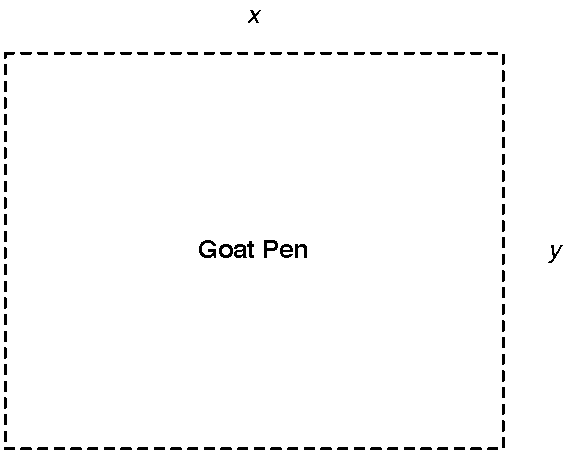
\includegraphics[scale=0.6]{imported_figures/GoatPen.pdf}
\caption{Goat pen with unknown side lengths. The objective is to identify the values of $x$ and $y$ that maximize the area of the pen (and thus the number of goats that can be kept).}
\label{fig:GoatPen}
\end{figure}
Clearly, we know that:
\begin{equation}
2x + 2y = 100
\label{eqn:GoatPerimeter}
\end{equation}
because $2x + 2y$ is the perimeter of the pen and I have 100 meters of fencing to build my pen. The area of the pen is $A(x,y) = xy$. We can use Equation \ref{eqn:GoatPerimeter} to solve for $x$ in terms of $y$. Thus we have:
\begin{equation}
y = 50 - x
\end{equation}
and $A(x) = x(50-x)$. To maximize $A(x)$, recall we take the first derivative of $A(x)$ with respect to $x$, set this derivative to zero and solve for $x$:
\begin{equation}
\frac{dA}{dx} = 50-2x = 0;
\end{equation}
Thus, $x = 25$ and $y = 50-x = 25$. We further recall from basic calculus how to confirm that this is a maximum; note:
\begin{equation}
\left.\frac{d^2A}{dx^2}\right|_{x = 25} = -2 < 0
\end{equation}
Which implies that $x = 25$ is a \term{local maximum} for this function. Another way of seeing this is to note that $A(x) = 50x-x^2$ is an concave (a frowning parabola). As we could have guessed, a square will maximize the area available for holding goats. 

We can re-write the problem to be in a more common form
\begin{equation}
\left\{
\begin{aligned}
\max \;\; & A(x,y) = x y \\
s.t. \;\; & 2x + 2y = 100 \equiv 2x + 2y - 100 = 0\\
& x \geq 0 \equiv -x \leq 0\\
& y \geq 0 \equiv -y \leq 0 
\end{aligned}\right.
\label{eqn:GoatMax}
\end{equation}
Note we've added two inequality constraints $x \geq 0$ and $y \geq 0$ because it doesn't really make any sense to have negative lengths. In our problem, we now have: $g_1(x,y) = -x$ and $g_2(x,y) = -y$ and $h(x,y) = 2x+2y-100$ to be consistent with the notation in Theorem \ref{thm:KKT7}. It is worth noting, we could have used the constraint $2x + 2y - 100 \leq 0$ instead and obtained the same answer.

For the point of optimality ($x=25$, $y=25$), let us now compute the KKT conditions. Note first:
\begin{equation}
\nabla A = \begin{bmatrix}y\\x\end{bmatrix} \quad \quad 
\nabla h = \begin{bmatrix}2\\2\end{bmatrix} \quad \quad 
\nabla g_1 = \begin{bmatrix}-1\\0\end{bmatrix} \quad \quad 
\nabla g_2 = \begin{bmatrix}0\\-1\end{bmatrix} \quad \quad 
\end{equation}
Substituting $x^* = y^* = 25$, we can see that primal feasibility is obviously satisfied. Moreover:
\begin{equation}
\nabla A(x^*,y^*) = \begin{bmatrix}25\\25\end{bmatrix}
\end{equation}
We  consider only dual feasibility and complimentary slackness. 
\begin{gather*}
\text{Dual Feasibility}:\left\{
\begin{aligned}
\begin{bmatrix}25\\25\end{bmatrix} -\lambda_1\begin{bmatrix}-1\\0\end{bmatrix} - 
\lambda_2\begin{bmatrix}0\\-1\end{bmatrix} - \mu\begin{bmatrix}2\\2\end{bmatrix} &= \begin{bmatrix}0\\0\end{bmatrix}\\
\lambda_1,\lambda_2 & \geq 0\\
\mu &\in \mathbb{R}
\end{aligned}
\right.\\
\text{Complementary Slackness}:\left\{
\begin{aligned}
\lambda_1(-x^*) = \lambda_1\cdot(-25) &= 0\\
\lambda_2(-y^*) = \lambda_2\cdot(-25) &= 0
\end{aligned}
\right.
\end{gather*}
Notice we substituted $x^*$ and $y^*$ into the complementary slackness equations. From complementary slackness, we see at once that $\lambda_1 = \lambda_2 = 0$. This means dual feasibility reduces to:
\begin{equation}
\begin{bmatrix}25\\25\end{bmatrix} - \mu\begin{bmatrix}2\\2\end{bmatrix} = \begin{bmatrix}0\\0\end{bmatrix}
\end{equation}
The solution: $\mu = 25/2$ satisfies this equality. Notice the gradient of the objective and the gradient of the (single) binding constraint are parallel. Notice also unlike a linear programming problem, the optimal solution to this problem \term{does not} occur at the extreme point of the constraint set (which is really just the line segment $2x + 2y = 100$ with $x,y\geq 0$). This geometric interpretation is illustrated in Figure \ref{fig:KKTNLP}. The gradient of the objective is shown in red, the gradient of the binding constraint is shown in green. Note, the gradient of the binding constraint has been scaled for visual effect. As expected, the level curves shown are given by the (implicit) equation $xy = k$. As you go up and right, the value of $k$ increases.
\begin{figure}[htbp]
\centering
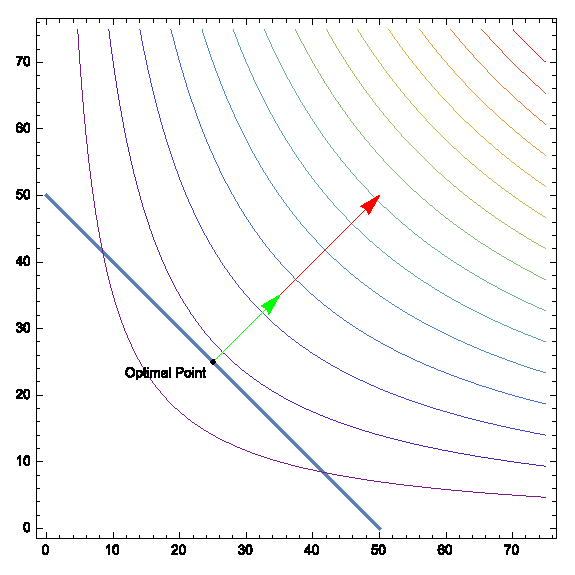
\includegraphics[scale=0.75]{imported_figures/KKTNLP.eps}
\caption{Visualization of the KKT conditions for a simple nonlinear programming problem. Notice the point of optimality is not at an extreme point. Moreover, the gradient of the binding constraint is parallel to the gradient of the objective, as expected. \term{Note, the gradient of the binding constraint has been scaled larger for visual effect.}}
\label{fig:KKTNLP}
\end{figure}

\section[Supplementary Material: KKT Conditions]{Supplementary Material: KKT Conditions \footnote{These notes are taken from \href{https://www.stat.cmu.edu/~ryantibs/convexopt/}{Machine Learning 10-725 (Convex Optimization)}.}}


\subsection{Dual Problem}

Given the following convex minimization problem:

\begin{problem}[convex minimization problem]
    \label{pro:kkt-problem}
    \begin{equation}
\begin{array}{ll}
\min _{x} & f(x) \\
\text { subject to } & h_{i}(x) \leq 0, \quad i=1, \ldots, m \\
& \ell_{j}(x)=0, \quad j=1, \ldots, r
\end{array}
\end{equation}
The Lagrangian is defined as $ L(x, u, v)=f(x)+\sum_{u=1}^{m} u_{i} h_{i}(x)+\sum_{j=1}^{r} v_{j} \ell_{j}(x) . $ The Lagrange dual function is defined as $ g(u, v)=\min _{x} L(x, u, v) $. The dual problem is
\begin{equation}
\begin{array}{ll}
\max _{u, v} & g(u, v) \\
\text { subject to } & u \geq 0
\end{array}
\end{equation}
\end{problem}


The Lagrange dual function $ g(u, v) $ is always \term{concave} regardless of whether the primal problem is convex or not.

\term{Weak duality}: $ f^{*} \geq g^{*} $ holds for all problems, where $ f^{*} $ and $ g^{*} $ are primal and dual optimal values, respectively.

Slaters's condition, which says the primal has at least one strictly feasible point, is a sufficient condition for \term{strong duality} to hold. If $ \exists x $ such that $ h_{i}(x)<0, i=1, \ldots, m $ and $ \ell_{j}(x)=0, j=1, \ldots, r, f^{*}=g^{*} $. This condition can be further refined to $ h_{i}(x)<0 $ for all $ i $ such that $ h_{i} $ is nonaffine. As a result, Slater's condition is reduced to feasibility for LP's.

\section{Karush-Kuhn-Tucker (KKT) Conditions}

For the given problem \ref{pro:kkt-problem}, the KKT conditions are:

\begin{enumerate}
    \item $ 0 \in \partial_{x}\left(f(x)+\sum_{i=1}^{m} u_{i} h_{i}(x)+\sum_{j=1}^{r} v_{j} \ell_{j}(x)\right) $ (stationary)
    \item $ u_{i} \cdot h_{i}(x)=0 $ for all $ i $ (complementary slackness)
    \item $ h_{i}(x) \leq 0, \ell_{j}(x)=0 $ for all $ i, j $ (primal feasibility)
    \item $ u_{i} \geq 0 $ for all $ i $ (dual feasibility)
\end{enumerate}

\begin{theorem}
    \label{thm:kkt-sufficient}
    For $ x^{*} $ and $ u^{*}, v^{*} $ to be primal and dual solutions, KKT conditions are sufficient.
\end{theorem}

\begin{proof}
    Sufficiency: if $ \exists x^{*} $ and $ u^{*}, v^{*} $ that satisfy the KKT conditions, $ g\left(u^{*}, v^{*}\right)=f\left(x^{*}\right)+\sum_{i=1}^{m} u_{i}^{*} h_{i}\left(x^{*}\right)+ $ $ \sum_{j=1}^{r} v_{j}^{*} \ell_{j}\left(x^{*}\right)=f\left(x^{*}\right) $ 
    
    The first equality holds from stationarity, since $ f(x)+\sum_{i=1}^{m} u_{i} h_{i}(x)+\sum_{j=1}^{r} v_{j} \ell_{j}(x) $ is convex, so any stationary point is a minimizer, and the second holds by complementary slackness. 
    
    By weak duality, $ x^{*} $ and $ u^{*}, v^{*} $ are optimal. It always implies that the duality gap is 0 .
\end{proof}

\begin{theorem}
    For a problem with strong duality (e.g. assume Slater's condition: convex problem and there exists $ x $ strictly satisfying nonaffine inequality constraints),

    $ x^{*} $ and $ u^{*}, v^{*} $ are primal and dual solutions $ \Longleftrightarrow x^{*} $ and $ u^{*}, v^{*} $ satisfy the KKT conditions
\end{theorem}


\begin{proof}

    Sufficiency: Follows from Theorem \ref{thm:kkt-sufficient}.


    Necessity: Let $ x^{*} $ and $ u^{*}, v^{*} $ be primal and dual solutions, and suppose we know strong duality holds.Then

    \begin{equation}
    \begin{aligned}
    f\left(x^{*}\right) &=g\left(u^{*}, v^{*}\right) \\
    &=\min _{x}\left(f(x)+\sum_{i=1}^{m} u_{i}^{*} h_{i}(x)+\sum_{j=1}^{r} v_{j}^{*} \ell_{j}(x)\right) \\
    & \leq f\left(x^{*}\right)+\sum_{i=1}^{m} u_{i}^{*} h_{i}\left(x^{*}\right)+\sum_{j=1}^{r} v_{j}^{*} \ell_{j}\left(x^{*}\right) \\
    & \leq f\left(x^{*}\right)
    \end{aligned}
    \end{equation}

The LSH equals RHS, so all inequalities in the equation must be equalities. Looking at the KKT conditions one by one, primal and dual feasibility holds, by virtue of optimality. Stationarity comes from the fact that $ x^{*} $ minimizes $ f(x)+\sum_{i=1}^{m} u_{i}^{*} h_{i}(x)+\sum_{j=1}^{r} v_{j}^{*} \ell_{j}(x) $. Since $ x^{*} $ is the minimizer, it must be a stationary point for this function. Complementary slackness comes from $ f\left(x^{*}\right)+\sum_{i=1}^{m} u_{i}^{*} h_{i}\left(x^{*}\right)+\sum_{j=1}^{r} v_{j}^{*} \ell_{j}\left(x^{*}\right)=f\left(x^{*}\right) $, since we must have $ \sum_{i=1}^{m} u_{i}^{*} h_{i}\left(x^{*}\right)=0 $ and they are each non-negative.

\end{proof}